%%%%%%%%%%%%%%%%%%%%%%%%%%%%%%%%%%%%%%%%%
% Journal Article
% LaTeX Template
% Version 1.4 (15/5/16)
%
% This template has been downloaded from:
% http://www.LaTeXTemplates.com
%
% Original author:
% Frits Wenneker (http://www.howtotex.com) with extensive modifications by
% Vel (vel@LaTeXTemplates.com)
%
% License:
% CC BY-NC-SA 3.0 (http://creativecommons.org/licenses/by-nc-sa/3.0/)
%
%%%%%%%%%%%%%%%%%%%%%%%%%%%%%%%%%%%%%%%%%

%----------------------------------------------------------------------------------------
%	PACKAGES AND OTHER DOCUMENT CONFIGURATIONS
%----------------------------------------------------------------------------------------

\documentclass[draft]{article}

\usepackage[utf8]{inputenc}
\usepackage{amsmath}
\usepackage{graphicx}
\usepackage{mhchem}

\usepackage{blindtext} % Package to generate dummy text throughout this template 

\usepackage[sc]{mathpazo} % Use the Palatino font
\usepackage[T1]{fontenc} % Use 8-bit encoding that has 256 glyphs
\linespread{1.05} % Line spacing - Palatino needs more space between lines
\usepackage{microtype} % Slightly tweak font spacing for aesthetics

\usepackage[english]{babel} % Language hyphenation and typographical rules


\usepackage[hmarginratio=1:1,top=32mm,columnsep=20pt]{geometry} % Document margins
\usepackage[hang, footnotesize,labelfont=bf,up,textfont=it,up]{caption} % Custom captions under/above floats in tables or figures
\usepackage{booktabs} % Horizontal rules in tables

\usepackage{lettrine} % The lettrine is the first enlarged letter at the beginning of the text

\usepackage{enumitem} % Customized lists
\setlist[itemize]{noitemsep} % Make itemize lists more compact

\usepackage{abstract} % Allows abstract customization
\renewcommand{\abstractnamefont}{\normalfont\bfseries} % Set the "Abstract" text to bold
\renewcommand{\abstracttextfont}{\normalfont\small\itshape} % Set the abstract itself to small italic text

\usepackage{titlesec} % Allows customization of titles
\renewcommand\thesection{\Roman{section}} % Roman numerals for the sections
\renewcommand\thesubsection{\roman{subsection}} % roman numerals for subsections
\titleformat{\section}[block]{\large\scshape\centering}{\thesection.}{1em}{} % Change the look of the section titles
\titleformat{\subsection}[block]{\large}{\thesubsection.}{1em}{} % Change the look of the section titles

\usepackage{fancyhdr} % Headers and footers
%\pagestyle{fancy} % All pages have headers and footers
\fancyhead{} % Blank out the default header
\fancyfoot{} % Blank out the default footer
%\fancyhead[C]{Running title $\bullet$ May 2016 $\bullet$ Vol. XXI, No. 1} % Custom header text
%\fancyfoot[RO,LE]{\thepage} % Custom footer text

\usepackage{titling} % Customizing the title section

\usepackage{hyperref} % For hyperlinks in the PDF

%----------------------------------------------------------------------------------------
%	TITLE SECTION
%----------------------------------------------------------------------------------------

\setlength{\droptitle}{-4\baselineskip} % Move the title up

\pretitle{\begin{center}\huge\bfseries} % Article title formatting
\posttitle{\end{center}} % Article title closing formatting
\title{A Mathematical Model for Calcium Release Via Ryanodine Receptors and Calcium-Calsequestrin Dynamics in Smooth Muscle Cells \\  \Large Master's Degree Research Proposal}
% Article title
\author{%
\textsc{Laura Sánchez Gómez} \\ % Your name
\normalsize CINVESTAV Monterrey \\ % Your institution
%\normalsize \href{mailto:john@smith.com}{john@smith.com} % Your email address
%\and % Uncomment if 2 authors are required, duplicate these 4 lines if more
%\textsc{Jane Smith}\thanks{Corresponding author} \\[1ex] % Second author's name
%\normalsize University of Utah \\ % Second author's institution
%\normalsize \href{mailto:jane@smith.com}{jane@smith.com} % Second author's email address
} % Leave empty to omit a date
\newcommand{\Cai}{[Ca^{2+}]_{i}}
\newcommand{\Cal}{[Ca^{2+}]_{SR}}
\newcommand{\al}{\textit{et al.} }
\newcommand{\ie}{\textit{i.e.} }
\newcommand{\eg}{\textit{e.g.} }
\renewcommand{\maketitlehookd}{%

\begin{otherlanguage}{english}
\begin{abstract}
\noindent Pendiente
\end{abstract}
\end{otherlanguage}
}

%----------------------------------------------------------------------------------------

\begin{document}
% Print the title
\maketitle

%----------------------------------------------------------------------------------------
%	ARTICLE CONTENTS
%----------------------------------------------------------------------------------------

\section{Introduction}

\lettrine[nindent=0em,lines=3]{C}
alcium is of great importance to cells. It participates in different processes such as proliferation, contraction, relaxation and apoptosis. rComo segundo mensajero, se encarga de transmitir información al interior de la célula desde la superficie. Dichos procesos son regulados por calcio mediante diferentes mecanismos de señalización que dependen de tiempo, espacio y amplitud. Entre ellos encontramos las chispas de calcio, que son aumentos de la concentración de calcio intracelular con una duración de milisegundos; los transitorios de calcio que se extienden a lo largo de todo el citoplasma con duración del orden de segundos; y las oscilaciones de calcio que son cambios globales en la concentración de calcio intracelular que presentan periodicidad compleja y tienen una duración de varios segundos e incluso minutos \cite{Perez-Rosas2016}. \\

Sin embargo, el exceso de calcio en el citoplasma resulta tóxico. Altas concentraciones de calcio intracelular producen agregación de proteínas y de ácidos nucleicos comprometiendo la membrana plasmática y produciendo precipitación de fosfatos \cite{Perez-Rosas2016}. Debido a esto, la célula invierte una gran cantidad de energía en mantener los niveles de calcio libre en citoplasma, alrededor de los 100 nM. Como el calcio no puede ser químicamente alterado, la célula debe quelarlo, compartimentarlo o extruirlo. Para ello, existen diferentes mecanismos  como bombas, canales, intercambiadores y proteínas amortiguadoras \cite{Carafoli2003}, \cite{Clapham2007}. \\

El calcio que entra al citoplasma proviene del medio extracelular y de un compartimento interno de la célula denominado retículo endoplásmico en células no musculares y retículo sarcoplásmico en células musculares. En la membrana plasmática se encuentran canales de calcio ligando dependientes y canales de calcio voltaje dependientes, que introducen calcio en la célula. Los encargados de extruír el calcio son los intercambiadores sodio/calcio y bombas PMCA (bomba de calcio ATPasa de la membrana plasmática). Por otro lado, en la membrana del retículo sarco/endoplásmico se encuentran embebidos canales de liberación de calcio como los RyRs (receptores de rianodina) y los IP$_3$Rs (receptores de inositol 1,4,5-trisfosfato); y la bomba SERCA (bomba de calcio ATPasa del retículo sarco/endoplásmico) encargada de rellenar el retículo. Adicional a esto, dentro del retículo se encuentran diferentes proteínas de unión a calcio que funcionan como amortiguadores del mismo \cite{Guerrero-Hernandez2010}, \cite{Carafoli2003}. \\

Las bombas PMCA y SERCA pertenecen a la familia de las ATPasas de tipo P, denominadas así porque se fosforilan durante el transporte. Cuentan con un dominio transmembranal y un dominio citosólico que contiene los sitios para hidrólisis de ATP y fosforilación. Estas bombas cuentan con dos estados conformacionales E1 y E2 y pasan de uno a otro durante el proceso de transporte. El estado E1 es abierto hacia el citosol y es más estable en la forma no fosforilada, momento durante el cual el calcio se une a la bomba. El estado E2 es abierto  hacia el espacio extracelular (en el caso de las bombas PMCA) o hacia el interior del retículo sarco/endoplásmico (en el caso de las bombas SERCA) y es más estable en la forma fosforilada, estado durante el cual el calcio es liberado \cite{Carafoli2003}, \cite{Perez-Rosas2016}. \\


Como se mencionó anteriormente, los canales encargados de la liberación de calcio desde el retículo sarco/endoplásmico son los IP$_3$Rs y  los RyRs. Los IP$_3$Rs son activados por  IP$_3$, el cual se produce mediante la siguiente cascada de señalización: en la membrana plasmática se encuentran receptores de tipo muscarínico, dichos receptores se encuentran acoplados a una proteína G. Cuando  el agonista se une al receptor, la subunidad $\alpha$ de la proteína G se disocia y activa la fosfolipasa C la cual hidroliza el PIP$_2$ (fosfatidilinositol 4,5-bifosfato) para producir IP$_3$ y DAG (diacilglicerol). Por su parte, los RyRs son activados mediante un mecanismo denominado CICR (liberación de calcio inducida por calcio por sus siglas en inglés). Un aumento en la concentración de calcio intracelular por encima de la concentración basal es sensada por los RyRs y se inicia la liberación de calcio proveniente del retículo sarco/endoplásmico  \cite{Kass1999}. \\


Dentro del retículo sarco/endoplásmico se encuentran diferentes proteínas de unión a calcio. Entre ellas la calsecuestrina, una proteína de alta capacidad y baja afinidad. Funciona como un amortiguador y le permite al retículo simultáneamente almacenar grandes cantidades de calcio en su interior y mantener la concentración de calcio luminal baja. Cuando la concentración de calcio luminal aumenta hasta alrededor de 1mM, la calsecuestrina comienza a polimerizarse formando primero dímeros, después tetrámeros y finalmente polímeros, aumentando su capacidad de almacenamiento \cite{Beard2004}, \cite{Park2004a}. \\

La concentración de calcio libre en los compartimentos de la célula (citoplasma y retículo sarco/endoplásmico) se cuantifica utilizando quelantes de calcio que aumentan su fluorescencia al unirse con él. En los experimentos que se mencionarán a continuación principalmente se utilizaron Fura-2 y Mag-Fluo4. Fura-2 utilizado para medir la concentración de calcio libre en citoplasma, es un fluoróforo que presenta alta afinidad por calcio ($K_d=0.23\mu M$). Emite fluorescencia al ser excitado con dos longitudes de onda diferentes ($340nm$ y $380nm$), lo que permite cuantificar la cantidad de calcio unido a él. Mag-Fluo4 usado para medir la concentración de calcio libre en el retículo sarcoplásmico, es un fluoróforo de baja afinidad por calcio ($K_d=22\mu M$). Emite fluorescencia al ser excitado con una sola longitud de onda ($390nm$), por lo tanto la cantidad de calcio unido se cuantifica en términos del aumento proporcional de su fluorescencia \cite{Takahashi1999}.


%------------------------------------------------

\section{Antecedentes}

Diferentes experimentos se han realizado para describir la dinámica de calcio dentro de la célula a partir de la liberación de este desde las pozas intracelulares. Dagnino-Acosta \al \cite{Dagnino-Acosta2009} observaron que tras estimular con $20 mM$ de cafeína, a un aumento en el calcio intracelular libre ($\Cai$) le correspondía una disminución en el calcio libre luminal ($\Cal$) como se muestra en la figura \ref{fig:FIGURA1}. Después de esperar $30$ segundos, se recuperaron los niveles basales de calcio en ambos compartimentos. Esto podría dar a entender que simplemente, el calcio pasó de un compartimento a otro. Sin embargo, al repetir la estimulación con $20 mM$  cafeína, se observó que la disminución en la $\Cal$ fue casi idéntica a la del primer estímulo, mientras que el aumento en la $\Cai$ fue muy pequeño en comparación, lo cual resulta contraintuitivo. Se requirió además de varios minutos para obtener una respuesta parcialmente similar a la del primer pulso. \\

\begin{figure}[h]
	\centering
	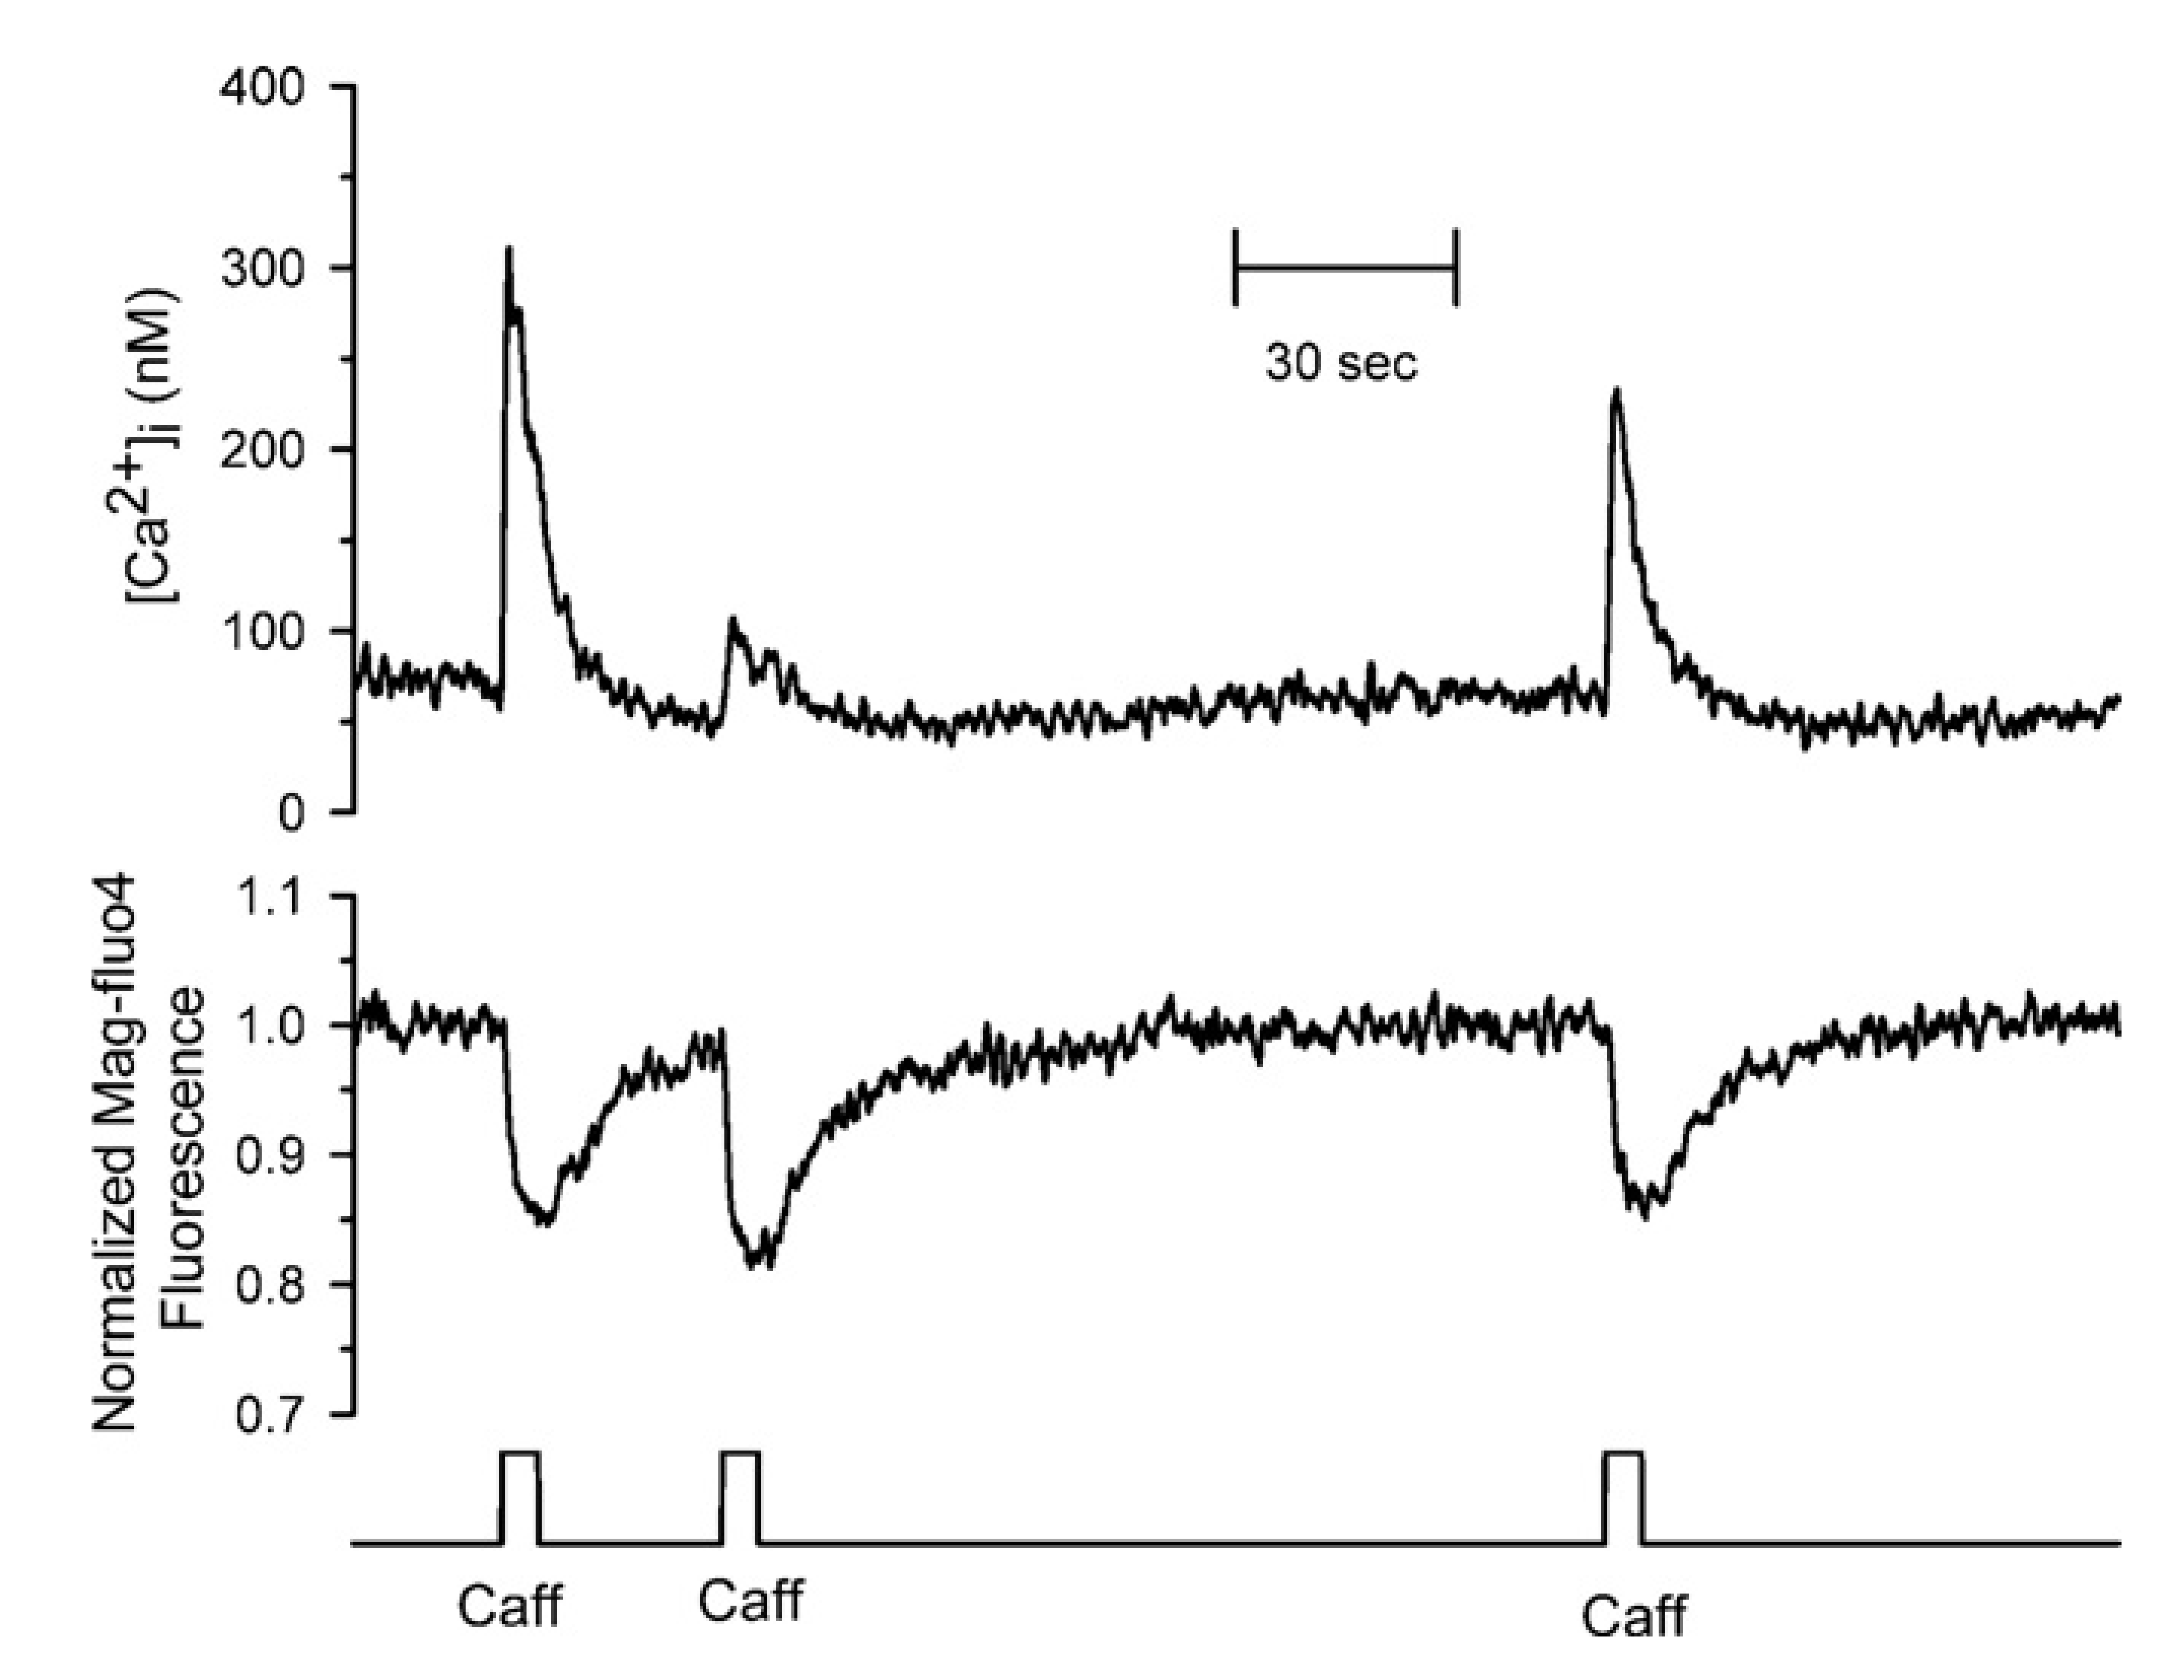
\includegraphics{FIGURA1}
	\caption{\textbf{Recuperación del retículo sarcoplásmico.} Registro simultáneo de la $\Cai$ y de la $\Cal$ en respuesta a estímulos de cafeína de $5$ segundos. Imagen tomada de la referencia \cite{Dagnino-Acosta2009}.}
	\label{fig:FIGURA1}
\end{figure}

Guerrero-Hernandez \al \cite{Guerrero-Hernandez2010} analizaron los planos fase de la $\Cal$ contra la $\Cai$ en diferentes tipos celulares (células aisladas de músculo liso, células de músculo esquelético, neuronas ganglionares aisladas de la raíz dorsal y células HeLa). La figura \ref{fig:FIGURA2}A muestra el plano fase para células de músculo liso, cuya liberación de calcio fue inducida por cafeína. Se pueden observar cuatro fases: la fase uno, momento en el cual se aplica el estímulo, se caracteriza por un aumento en la $\Cai$, sin mayor disminución en la $\Cal$; la fase dos por el contrario presenta una disminución en la $\Cal$, sin mayores cambios en la $\Cai$; la fase tres presenta una disminución en la $\Cai$ sin cambios en la $\Cal$; y por último, la fase cuatro muestra un aumento en la $\Cal$ sin cambios aparentes en la $\Cai$. La figura \ref{fig:FIGURA2}B muestra el plano fase para una chispa de calcio en células de músculo esquelético. Las fases uno y cuatro permanecen; sin embargo en contraste con el plano fase de células de músculo liso, las fases dos y tres se vuelven una sola, posiblemente debido a que los mecanismos de eliminación de calcio son muy rápidos. La figura \ref{fig:FIGURA2}C muestra el plano fase de la respuesta de calcio inducida por cafeína en neuronas ganglionares aisladas de la raíz dorsal, donde la fase uno ocurre sin cambios en la $\Cal$. Al igual que en el caso anterior, observamos que las fases dos y tres se unen como una sola fase, por la rapidez de los mecanismos de remoción de calcio. Finalmente, la figura \ref{fig:FIGURA2}D muestra el plano fase de la respuesta de calcio inducida por histamina en células HeLa. En este caso, se observan las fases uno y dos. Sin embargo, las fases tres y cuatro se ven como una sola, debido a que los mecanismos de remoción son muy lentos. \\

\begin{figure}[h]
	\centering
	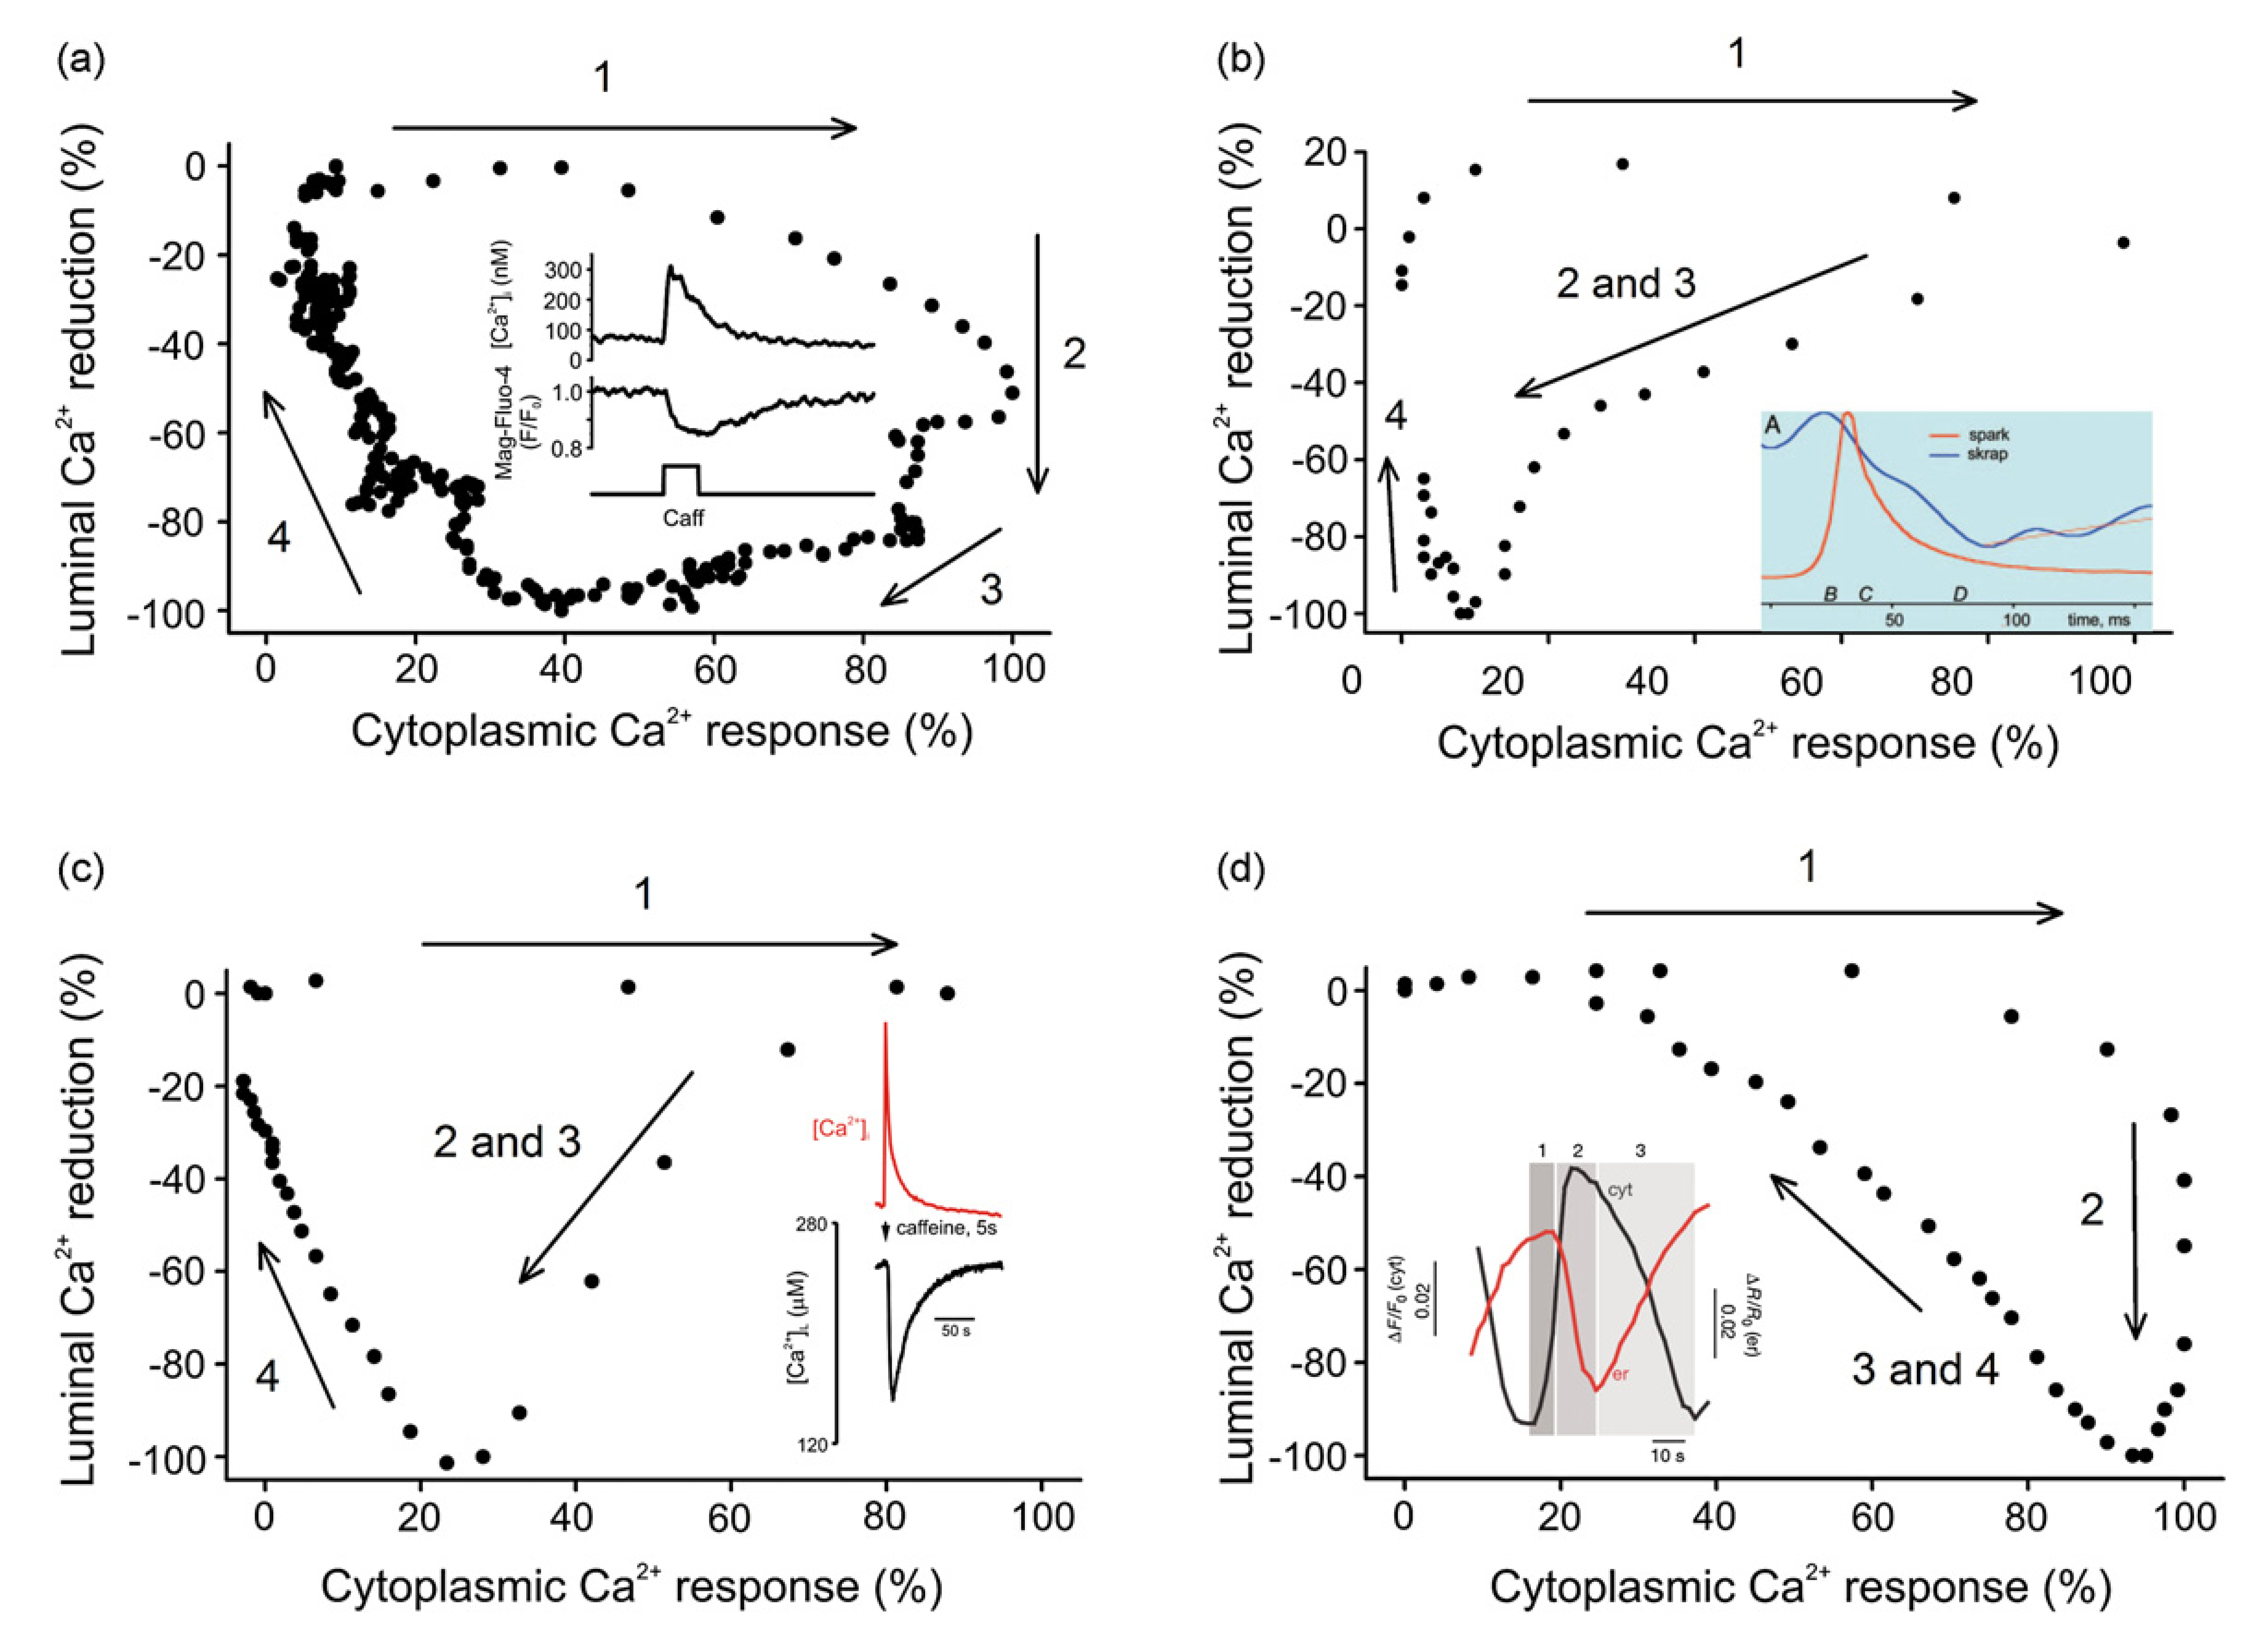
\includegraphics{FIGURA2}
	\caption{\textbf{Planos fase de la concentración de calcio en diferentes modelos celulares.} La imagen muestra los planos fase de la $\Cai$ contra la $\Cal$ en cuatro diferentes modelos celulares. Los recuadros muestran los datos utilizados para generar el plano fase. Imagen tomada de la referencia \cite{Guerrero-Hernandez2010}.}
	\label{fig:FIGURA2}
\end{figure}

Estos resultados concuerdan con la respuesta contraintuitiva de la figura \ref{fig:FIGURA1}. Por ello, los autores plantearon que el retículo sarco/endoplásmico tiene acceso a una fuente oculta de calcio, posiblemente relacionada con las proteínas de unión a calcio que en él se encuentran. La figura \ref{fig:FIGURA3} muestra los planos fase para cada uno de los pulsos de la figura \ref{fig:FIGURA1}. Aquí se observa que el retículo cuenta con un periodo refractario, el cual no se encuentra en fase con la recuperación de su nivel basal de calcio \cite{Guerrero-Hernandez2010}. \\

\begin{figure}[h]
	\centering
	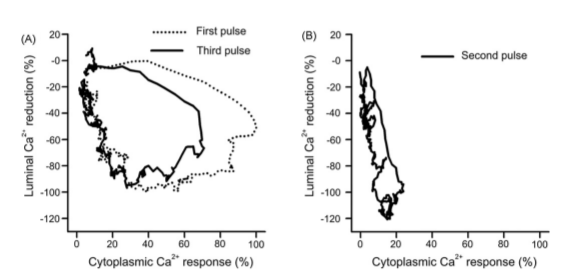
\includegraphics{FIGURA3}
	\caption{\textbf{Planos fase de la concentración de calcio en células de músculo liso.} La imagen muestra los planos fase de la $\Cai$ contra la $\Cal$ en células de músculo liso para cada uno de los tres pulsos de cafeína aplicados. Imagen tomada de la referencia \cite{Guerrero-Hernandez2010}.}
	\label{fig:FIGURA3}
\end{figure}

Park \al \cite{Park2004a} estudiaron la relación entre la unión de calcio con calsecuestrina y su polimerización. Para ello, utilizaron calsecuestrina proveniente de músculo esquelético de conejo (sCSQ), de músculo cardiaco de perro (cCSQ) y una calsecuestrina mutante($\Delta C27$). Esta última se obtuvo al eliminar los últimos 27 residuos de la calsecuestrina cardiaca. Para la cuantificación de calcio se utilizó espectroscopía de absorción atómica. Los resultados obtenidos se muestran en la figura \ref{fig:FIGURA9}. Se puede observar que la sCSQ presenta mayor capacidad de unión respecto a la cCSQ, mientras que la $\Delta C27$ presenta una capacidad de unión mucho menor que su equivalente nativa (superior al $50\%$). Además, el comportamiento de las calsecuestrinas nativas varía dependiendo de la concentración de calcio administrado, pues su capacidad amortiguadora parece aumentar conforme este aumenta. Más aun, la gráfica tipo Scatchard de la figura \ref{fig:FIGURA10}, muestra cómo varía la constante de disociación (representada por la pendiente) de calsecuestrina con calcio. Estos resultados refuerzan el hecho de que la capacidad amortiguadora del retículo varía dependiendo de la $\Cal$ como habían propuesto Guerrero-Hernandez \al \cite{Guerrero-Hernandez2010}. \\

\begin{figure}[h]
	\centering
	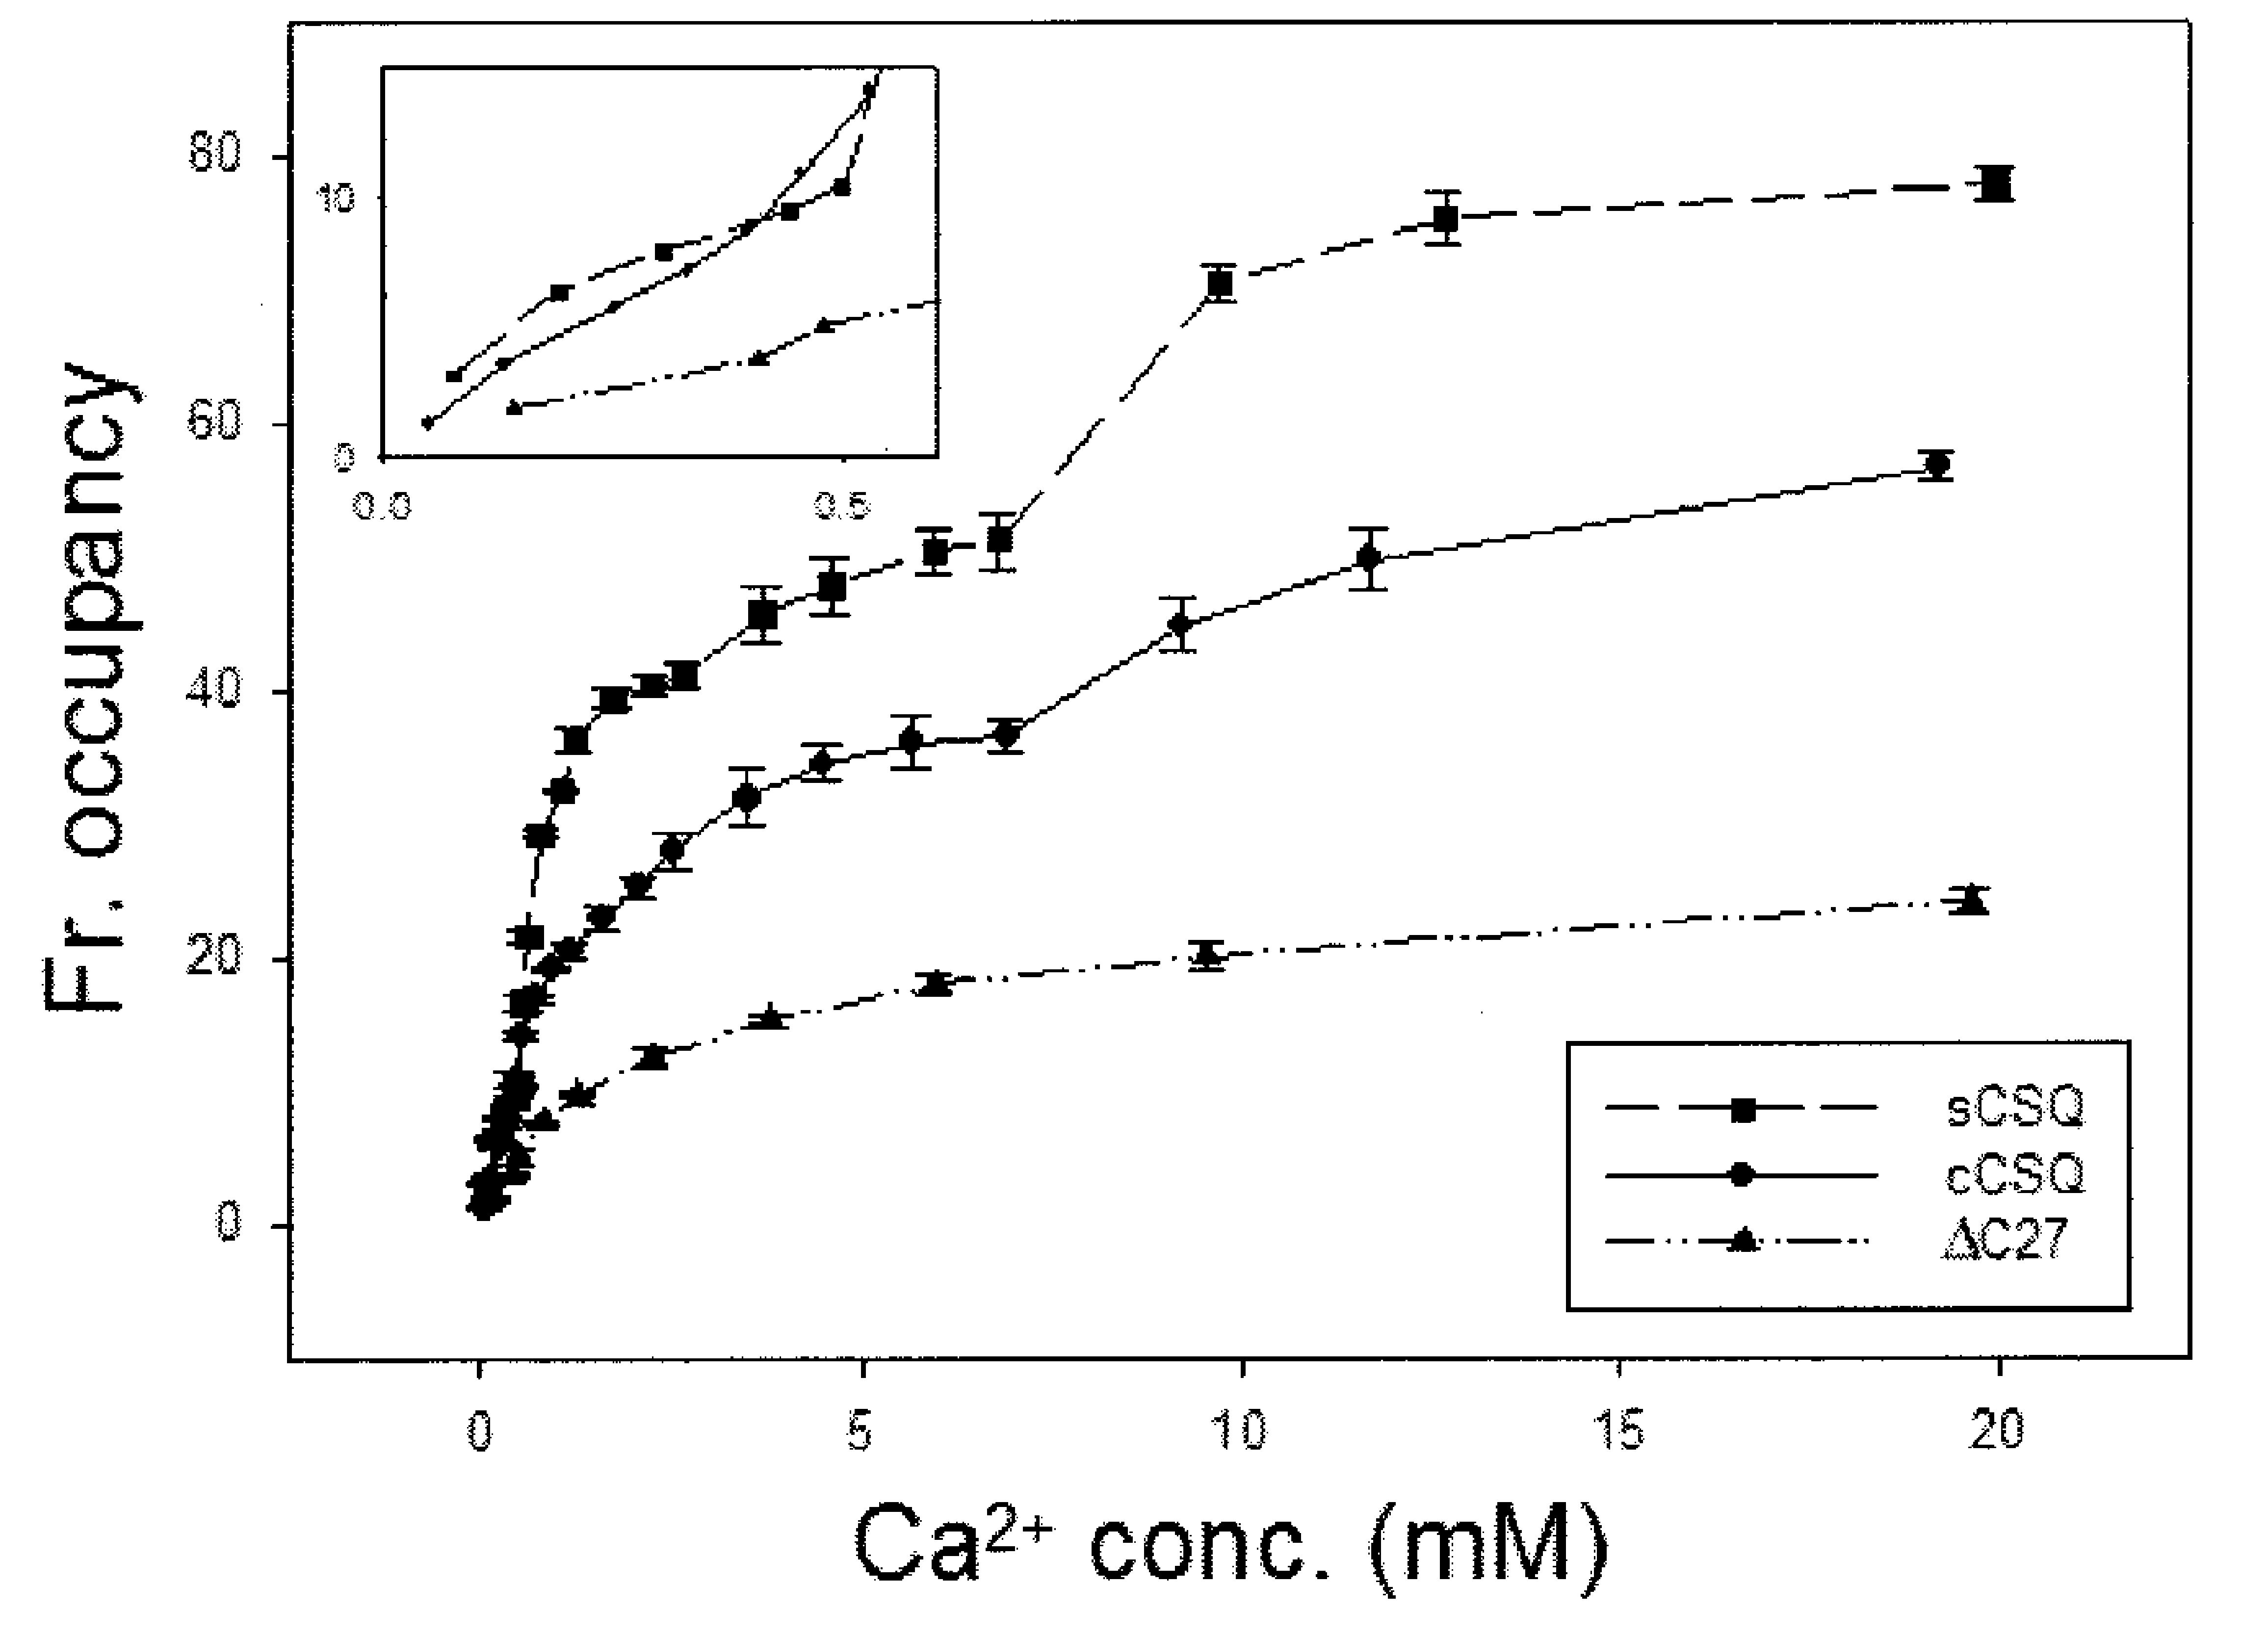
\includegraphics{FIGURA9}
	\caption{\textbf{Polimerización de la calsecuestrina.} La imagen muestra la polimerización de las proteínas nativas sCSQ, cCSQ y la dimerización de la proteína mutante $\Delta C27$. El acercamiento muestra la frecuencia ocupacional para concentraciones de calcio de $0 - 0.5 mM$. Imagen tomada de la referencia \cite{Park2004a}.}
	\label{fig:FIGURA9}
\end{figure}

\begin{figure}[h]
	\centering
	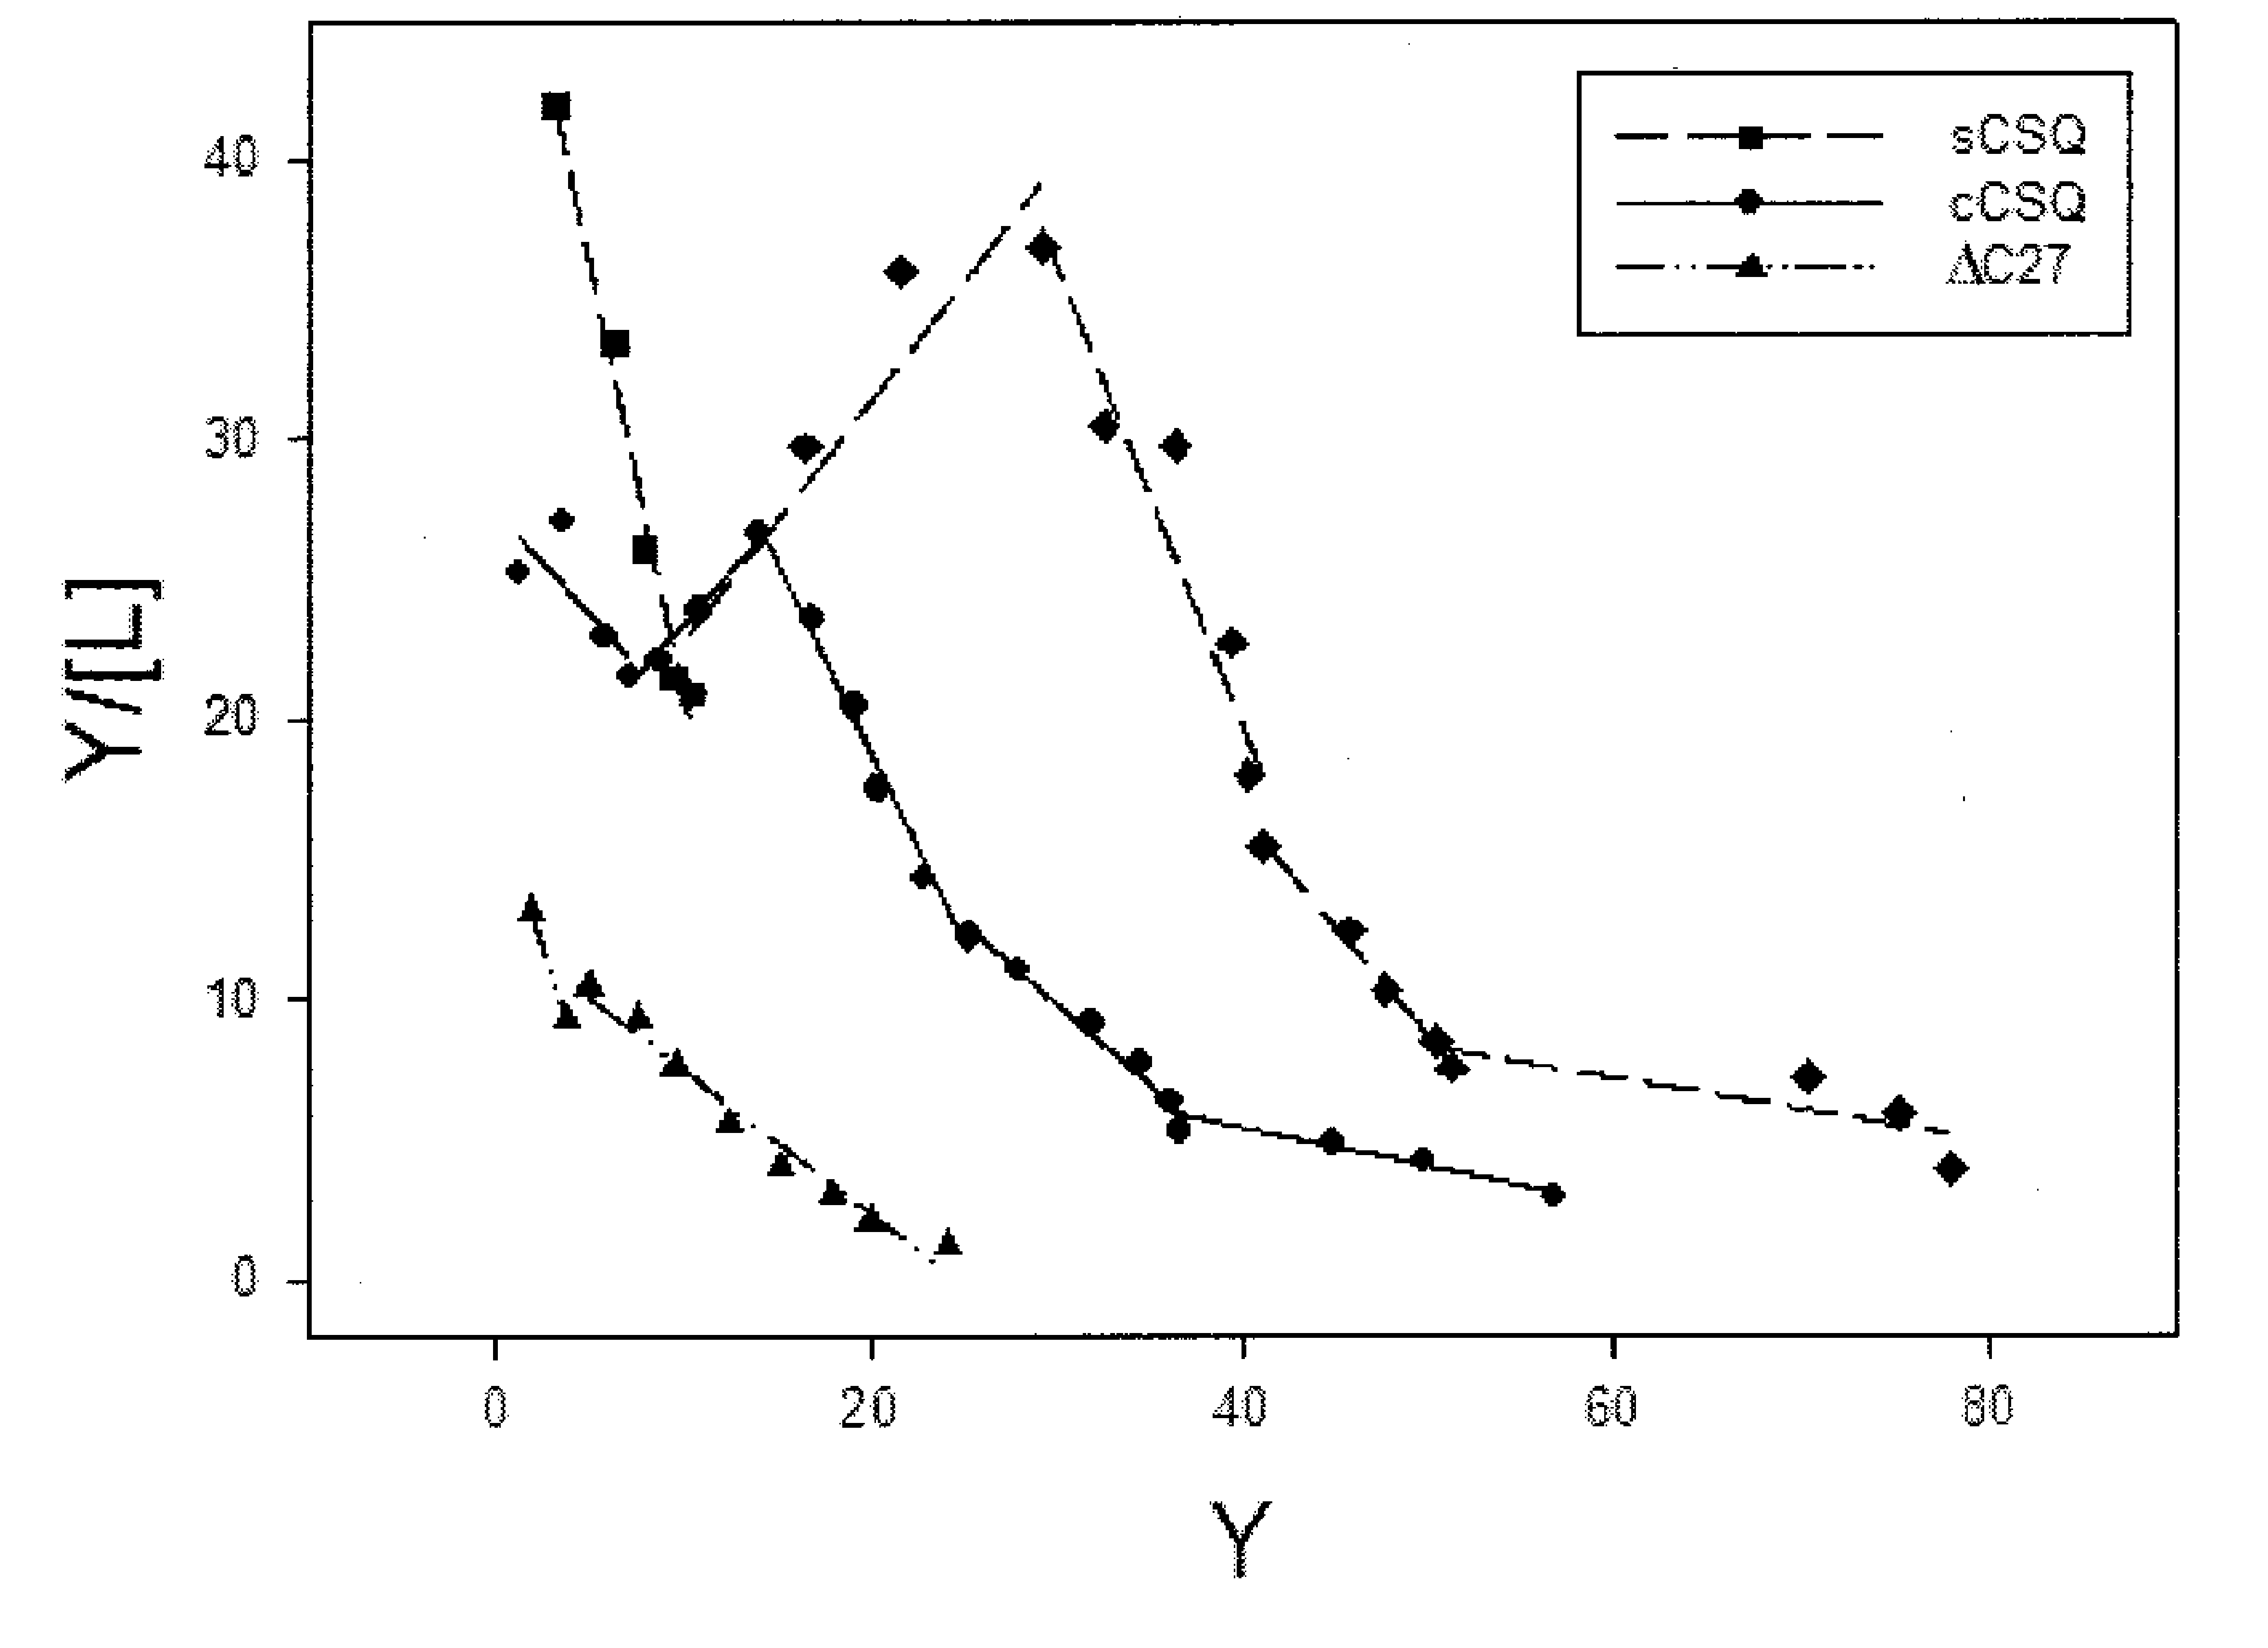
\includegraphics{FIGURA10}
	\caption{\textbf{Gráfica tipo Scatchard de la unión de calcio a calsecuestrina.} La gráfica muestra la variación en las constantes de disociación de calcio con calsecuestrina. Imagen tomada de la referencia \cite{Park2004a}.}
	\label{fig:FIGURA10}
\end{figure}

Debido a que la proteína mutante $\Delta C27$ podía formar dímeros, pero no polimerizarse más, los autores proponen que existe una relación entre la capacidad amortiguadora de la calsecuestrina y su polimerización. La figura \ref{fig:FIGURA11} muestra la capacidad amortiguadora tanto de cCSQ como de sCSQ cuando se encuentran como monómeros, dímeros, tetrámeros o polímeros en función de la concentración de calcio. Dado que la concentración de calcio para la cual las proteínas comienzan a polimerizarse es muy similar, se puede decir que dicha polimerización es inducida por la presencia de calcio. \\

\begin{figure}[h]
	\centering
	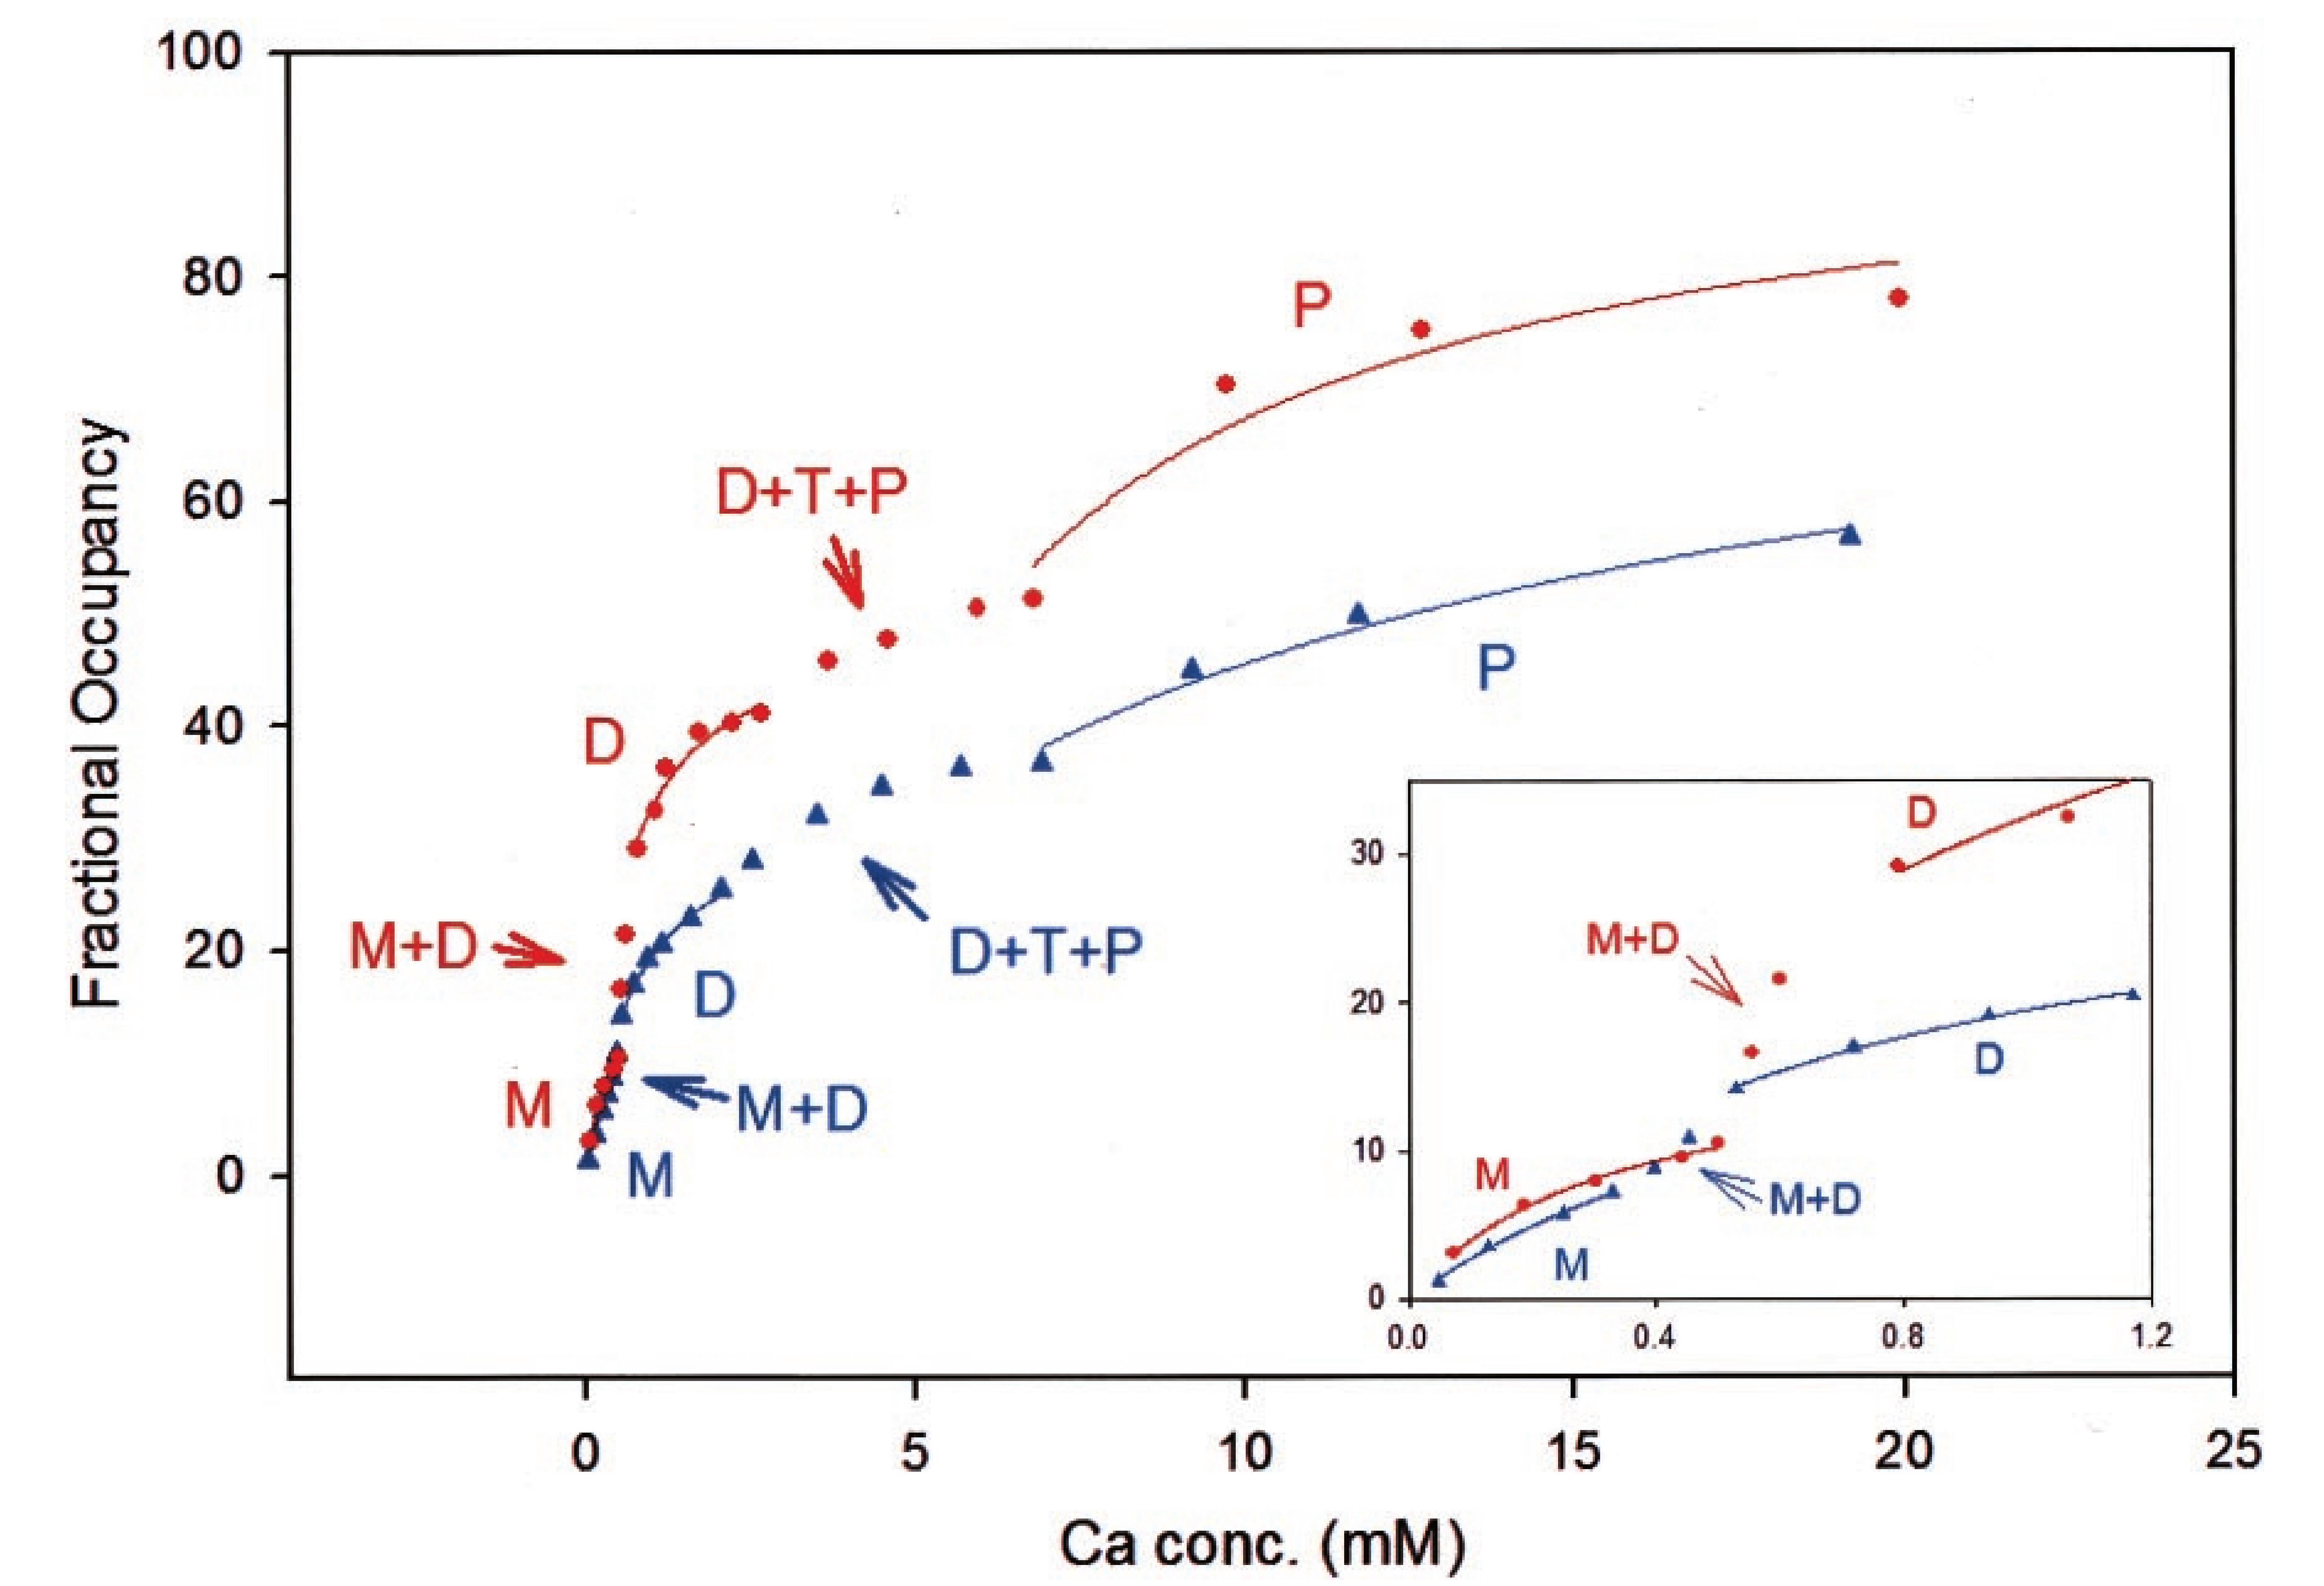
\includegraphics{FIGURA11}
	\caption{\textbf{Polimerización de la calsecuestrina.} La imagen muestra la concentración de calcio cuando la calsecuestrina forma monómeros (M), dímeros (D), tetrámeros (T) y polímeros (P). El acercamiento muestra la frecuencia ocupacional para concentraciones de calcio de $0 - 1.2 mM$. Imagen tomada de la referencia \cite{Park2004a}.}
	\label{fig:FIGURA11}
\end{figure}

En células de músculo liso de vejiga urinaria de conejillo de indias \cite{Perez-Rosas2015}, se indujo la liberación de calcio aplicando $20mM$ de cafeína durante $5$ segundos. Las concentraciones de calcio en citoplasma y en el retículo sarcoplásmico, se registraron simultáneamente en función del tiempo, como se muestra en la figura \ref{fig:FIGURA4}A. Se esperó a que se reestablecieran los valores basales de calcio en ambos compartimentos y posteriormente se procedió a bloquear las bombas SERCA aplicando $10\mu M$ de tapsigargina durante $5$ segundos. Pasados $20$ segundos, se aplicó otro pulso de $20mM$ de cafeína durante $5$ segundos. Los planos fase para cada uno de los pulsos se muestran en la figura \ref{fig:FIGURA4}B. \\

\begin{figure}[h]
	\centering
	\includegraphics{FIGURA4}
	\caption{\textbf{La liberación de calcio inducida por cafeína involucra 4 fases que depen- den de la actividad de la bomba SERCA.} A. $\Cai$ y la $\Cal$ en función del tiempo. B. Planos fase para cada uno de los pulsos de cafeína. Imagen tomada de la referencia \cite{Perez-Rosas2015}.}
	\label{fig:FIGURA4}
\end{figure}

En la figura \ref{fig:FIGURA4}A se observa que la adición de tapsigargina no modificó los niveles basales de calcio en ninguno de los compartimentos. Sin empargo, tras haber inhibido las bombas SERCA, el transitorio de calcio resulta ser de menor magnitud que el inducido por cafeína antes de aplicar la tapsigargina mientras que la disminución de la $\Cal$ es similar para ambos pulsos. Tras el segundo pulso, los niveles basales de calcio en el retículo no se recuperaron como era de esperarse. La figura \ref{fig:FIGURA4}B muestra las fases ya descritas anteriormente presentes en el primer pulso, en contraste con el plano fase graficado para el segundo pulso. En el segundo pulso las fases uno y dos desaparecen y se presenta una sola fase. Esta muestra un comportamiento lineal entre el aumento en la $\Cai$ y la disminución de la $\Cal$. Esto sugiere que las bombas SERCA juegan un papel fundamental en la liberación de calcio desde el retículo sarcoplásmico además de su ya conocida participación en el llenado del mismo. \\

Para explicar el aumento en la capacidad amortiguadora del retículo sarcoplásmico, Perez-Rosas \al \cite{Perez-Rosas2015} propusieron un modelo matemático el cual denominaron cinética bajo demanda (KonD por sus siglas en inglés). El modelo KonD explica la fase uno de la liberación de calcio del retículo sarcoplásmico, así como el periodo refractario asociado a la recuperación de la $\Cal$. KonD está basado en la hipótesis de que la cantidad de sitios de unión de las proteínas amortiguadoras aumenta conforme la $\Cal$ lo hace; esto en contraste con la cinética estándar (SK por sus siglas en inglés) en la que los sitios de unión permanecen constantes. Consideremos la siguiente reacción

\begin{equation*}
\ce{{[B_0]} + {\Cal} <=>[k^{+}_B][k^{-}_B] {[B_1]} }
\end{equation*}
 
donde $[B_0]$ representa la concentración de sitios de unión libres de calcio con calsecuestrina y $[B_1]$ la concentración de sitios ocupados. Analizando la reacción en el equilibrio químico, por la ley de acción de masas se tiene que

\begin{equation}\label{BS}
\frac{[B_0][Ca^{2+}]_{SR}}{[B_1]}= K_B
\end{equation}

donde $K_B = \frac{k^{-}_B}{k^{+}_B}$ es la constante de disociación de la reacción. Para el caso del modelo KonD el aumento de sitios de unión se representó con la siguiente ecuación, en la cual $[B_T]$ es la concentración total de sitios de unión,

\begin{equation}\label{BSKonD}
[B_0] = [B_T] + [B_1]
\end{equation}

mientras que para el modelo SK se representaron de la siguiente forma

\begin{equation}\label{BSSK}
[B_0] = [B_T] - [B_1].
\end{equation}

Ahora bien, la concentración total de calcio en el retículo ($[Ca^{2+}]_{TSR}$) se puede expresar como

\begin{equation}\label{CalcioTotal}
[Ca^{2+}]_{TSR} = \Cal + [B_1].
\end{equation}

De las ecuaciones \ref{BS}, \ref{BSKonD} y \ref{CalcioTotal} obtenemos que la $\Cal$ para el modelo KonD en función de la concentración total de calcio en el retículo esta dada por

\begin{equation}\label{KonD}
\Cal = \frac{1}{2} \xi - \frac{1}{2} \sqrt{\xi^2 - 4[Ca^{2+}]_{TSR}K_R}
\end{equation}

donde $\xi = [Ca^{2+}]_{TSR} + P_T + K_R$. De manera análoga, de las ecuaciones \ref{BS}, \ref{BSSK} y \ref{CalcioTotal} se tiene que para el modelo SK, la $\Cal$ está dada por

\begin{equation}\label{SK}
[Ca^{2+}]_{SR} = \frac{1}{2} \xi + \frac{1}{2} \sqrt{\xi^2 + 4[Ca^{2+}]_{TSR}K_R}
\end{equation}

donde $\xi = [Ca^{2+}]_{TSR} - P_T - K_R$. \\

La figura \ref{fig:FIGURA12} compara el comportan los sitios de unión de calsecuestrina a calcio según la SK (B) y la KonD (A). En el caso de la SK el número de sitios de unión de calcio con calsecuestrina es finito y eventualmente conforme va aumentando la $\Cal$ estos se saturan. Además, a medida que se va liberando calcio a través de los RyRs y los sitios de unión a calcio se van vaciando, comienzan a competir con los RyRs por el calcio luminal libre. Debido a esto, la SK no puede reproducir las fases uno y dos de la libración de calcio por parte del retículo sarcoplásmico y la transición entre ellas. Por el contrario, KonD propone que a medida que aumenta la $\Cal$, los sitios de unión de calcio con calsecuestrina también aumentan. Además, conforme el calcio se va despegando de la proteína de unión los sitios desaparecen. De esta forma no se presenta competencia alguna entre los RyRs y las proteínas de unión por el calcio luminal \cite{Perez-Rosas2016}. \\

\begin{figure}[h]
	\centering
	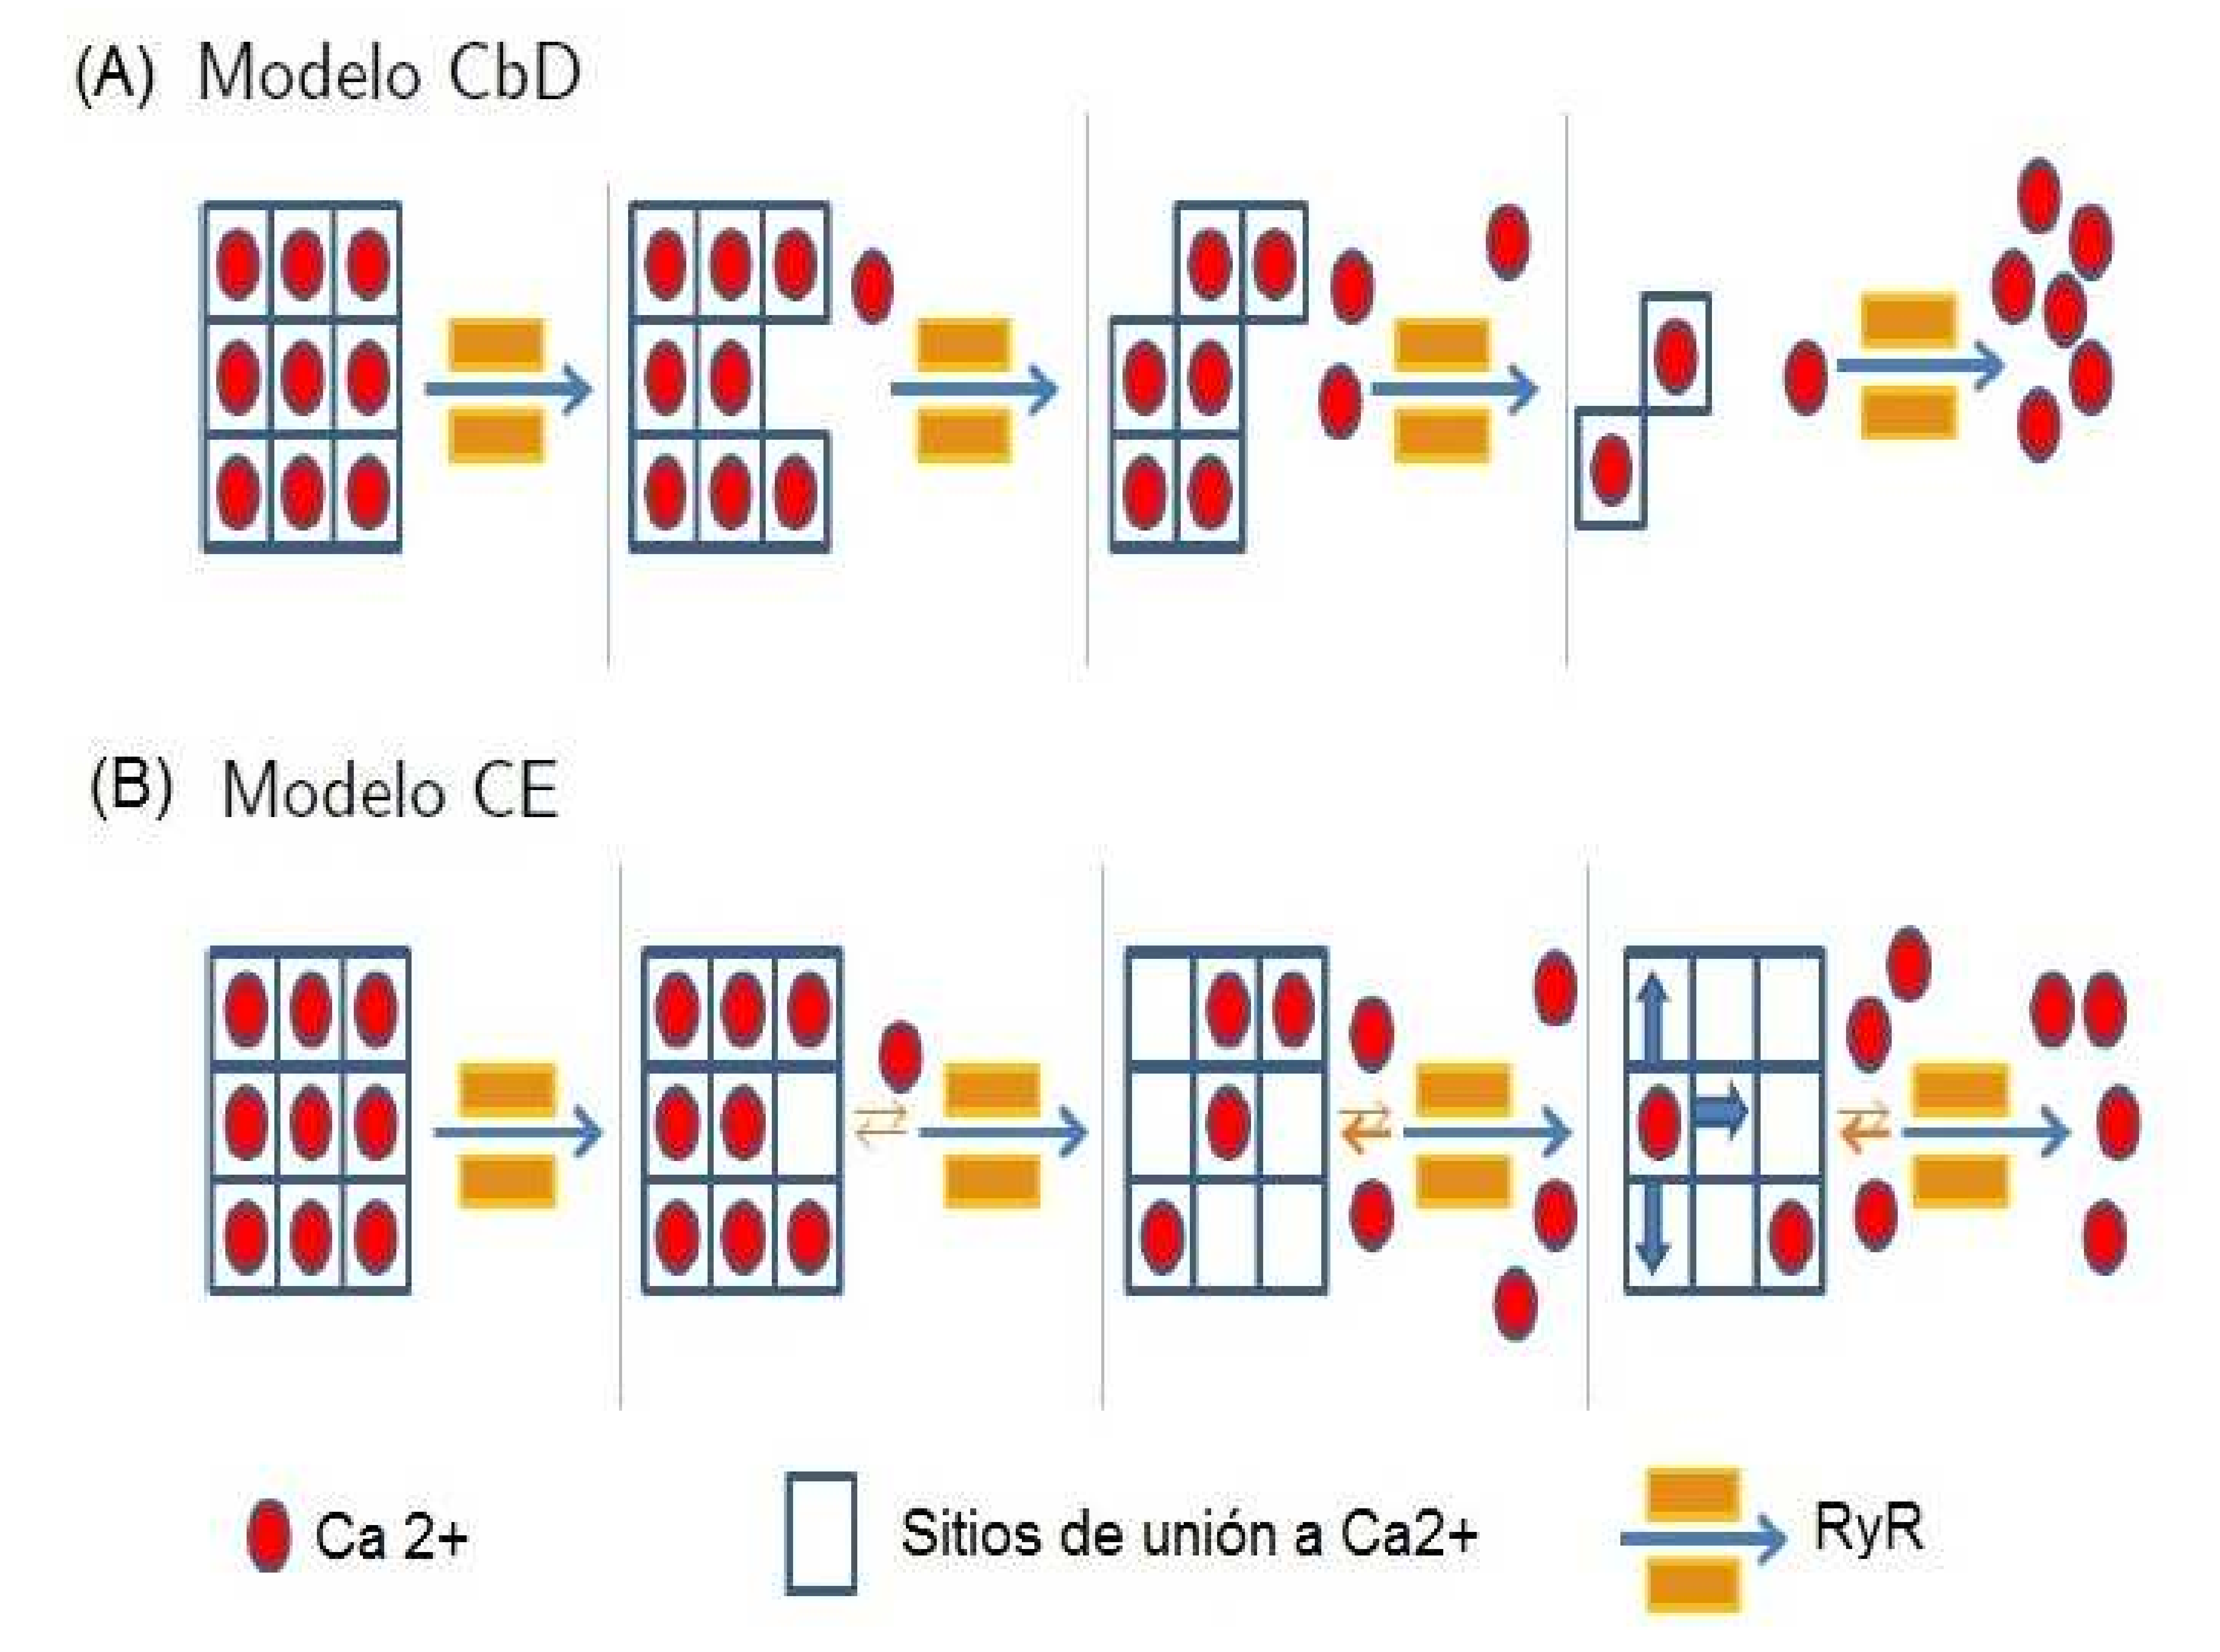
\includegraphics{FIGURA12}
	\caption{\textbf{Sitios de unión de calcio con calsecuestrestina según KonD y SK.} A. En la KonD, los sitios de unión aparecen y desaparecen conforme aumenta o disminuye la concentración de calcio luminal, respectivamente. B. En la SK hay un número finito de sitios de unión los cuales se saturan conforme aumenta la concentración de calcio luminal. Además, existe competencia entre los sitios de unión libres a medida que se libera calcio y los RyR.Imagen tomada de la referencia \cite{Perez-Rosas2016}.}
	\label{fig:FIGURA12}
\end{figure}

El modelo logró reproducir los pulsos inducidos por cafeína de $2mM$ y $20mM$ como lo muestran las figuras \ref{fig:FIGURA5} y \ref{fig:FIGURA6}, resprectivamente. La variabilidad obtenida en los experimentos se simuló asumiendo que el volumen del retículo que respondía al estímulo de cafeína variaba de $1\% - 10\%$ del volumen celular. Para ambos casos, el panel A muestra la amplitud y la velocidad máxima de la respuesta de calcio inducida por cafeína para 49 y 66 células (puntos), respectivamente y los valores obtenidos con el modelo (en azul); el panel B muestra la velocidad máxima de la $\Cai$ en función del tiempo; y el panel C muestra el curso temporal de la $\Cai$ (azul) el cual se ajusta a los valores experimentales obtenidos (círculos) y la $\Cal$ (verde) producto del pulso de de cafeína. \\

\begin{figure}[h]
	\centering
	\includegraphics{FIGURA5}
	\caption{\textbf{Respuesta de calcio inducida por 2mM de cafeína y simulación hecha con el modelo KonD.} A. La imagen muestra la variabilidad de la velocidad máxima en función de la concentración. B. Velocidad máxima en función del tiempo. C. Curso temporal de la $\Cai$, ajuste del modelo KonD y reducción de la $\Cal$ en función del tiempo. Imagen tomada de la referencia \cite{Perez-Rosas2015}.}
	\label{fig:FIGURA5}
\end{figure}

\begin{figure}[h]
	\centering
	\includegraphics{FIGURA6}
	\caption{\textbf{Respuesta de calcio inducida por 20mM de cafeína y simulación hecha con el modelo KonD.} A. La imagen muestra la variabilidad de la velocidad máxima en función de la concentración. B. Velocidad máxima en función del tiempo. C. Curso temporal de la $\Cai$, ajuste del modelo KonD y reducción de la $\Cal$ en función del tiempo. Imagen tomada de la referencia \cite{Perez-Rosas2015}.}
	\label{fig:FIGURA6}
\end{figure}

Más aun, mediante el mismo modelo, los autores pudieron reproducir la respuesta obtenida tras aplicar $5\mu M$ de tapsigargina, para bloquear las bombas SERCA, y posteriormente $20mM$ de cafeína. Los resultados se muestran en la figura \ref{fig:FIGURA7}. La figura \ref{fig:FIGURA7}A muestra la amplitud y la velocidad máxima de la respuesta de calcio inducida por cafeína (puntos) y los valores obtenidos con el modelo (en azul); la figura \ref{fig:FIGURA7}B muestra la velocidad máxima de la $\Cai$ en función del tiempo; y la figura \ref{fig:FIGURA7}C presenta el trazo temporal de la $\Cai$ obtenida experimentalmente (círculos), la $\Cai$ obtenienda con el modelo (azul) y la correspondiente $\Cal$ (verde). \\

\begin{figure}[h]
	\centering
	\includegraphics{FIGURA7}
	\caption{\textbf{Efecto de la inhibición de la bomba SERCA por tapsigargina en las respuestas del calcio intracelular inducidas al aplicar 20mM de cafeína.} A. La imagen muestra la variabilidad de la velocidad máxima en función de la concentración. B. Velocidad máxima en función del tiempo. C. Curso temporal de la $\Cai$, ajuste del modelo KonD y reducción de la $\Cal$ en función del tiempo. Imagen tomada de la referencia \cite{Perez-Rosas2015}.}
	\label{fig:FIGURA7}
\end{figure}

El modelo de KonD también fue capaz de representar el periodo refractario descrito por Guerrero-Hernandez \al \cite{Guerrero-Hernandez2010}. En el experimento se aplicó un pulso de cafeína, se esperó a que se recuperaran las concentraciones basales en los dos compartimentos y se aplicó otro pulso de cafeína. El segundo transitorio fue menor al obtenido después del primer pulso. La figura \ref{fig:FIGURA8} muestra la comparación entre la SK (verde) y la KonD (café) junto con los datos experimentales (azul), tanto para la $\Cai$ como para la $\Cal$. \\

\begin{figure}[h]
	\centering
	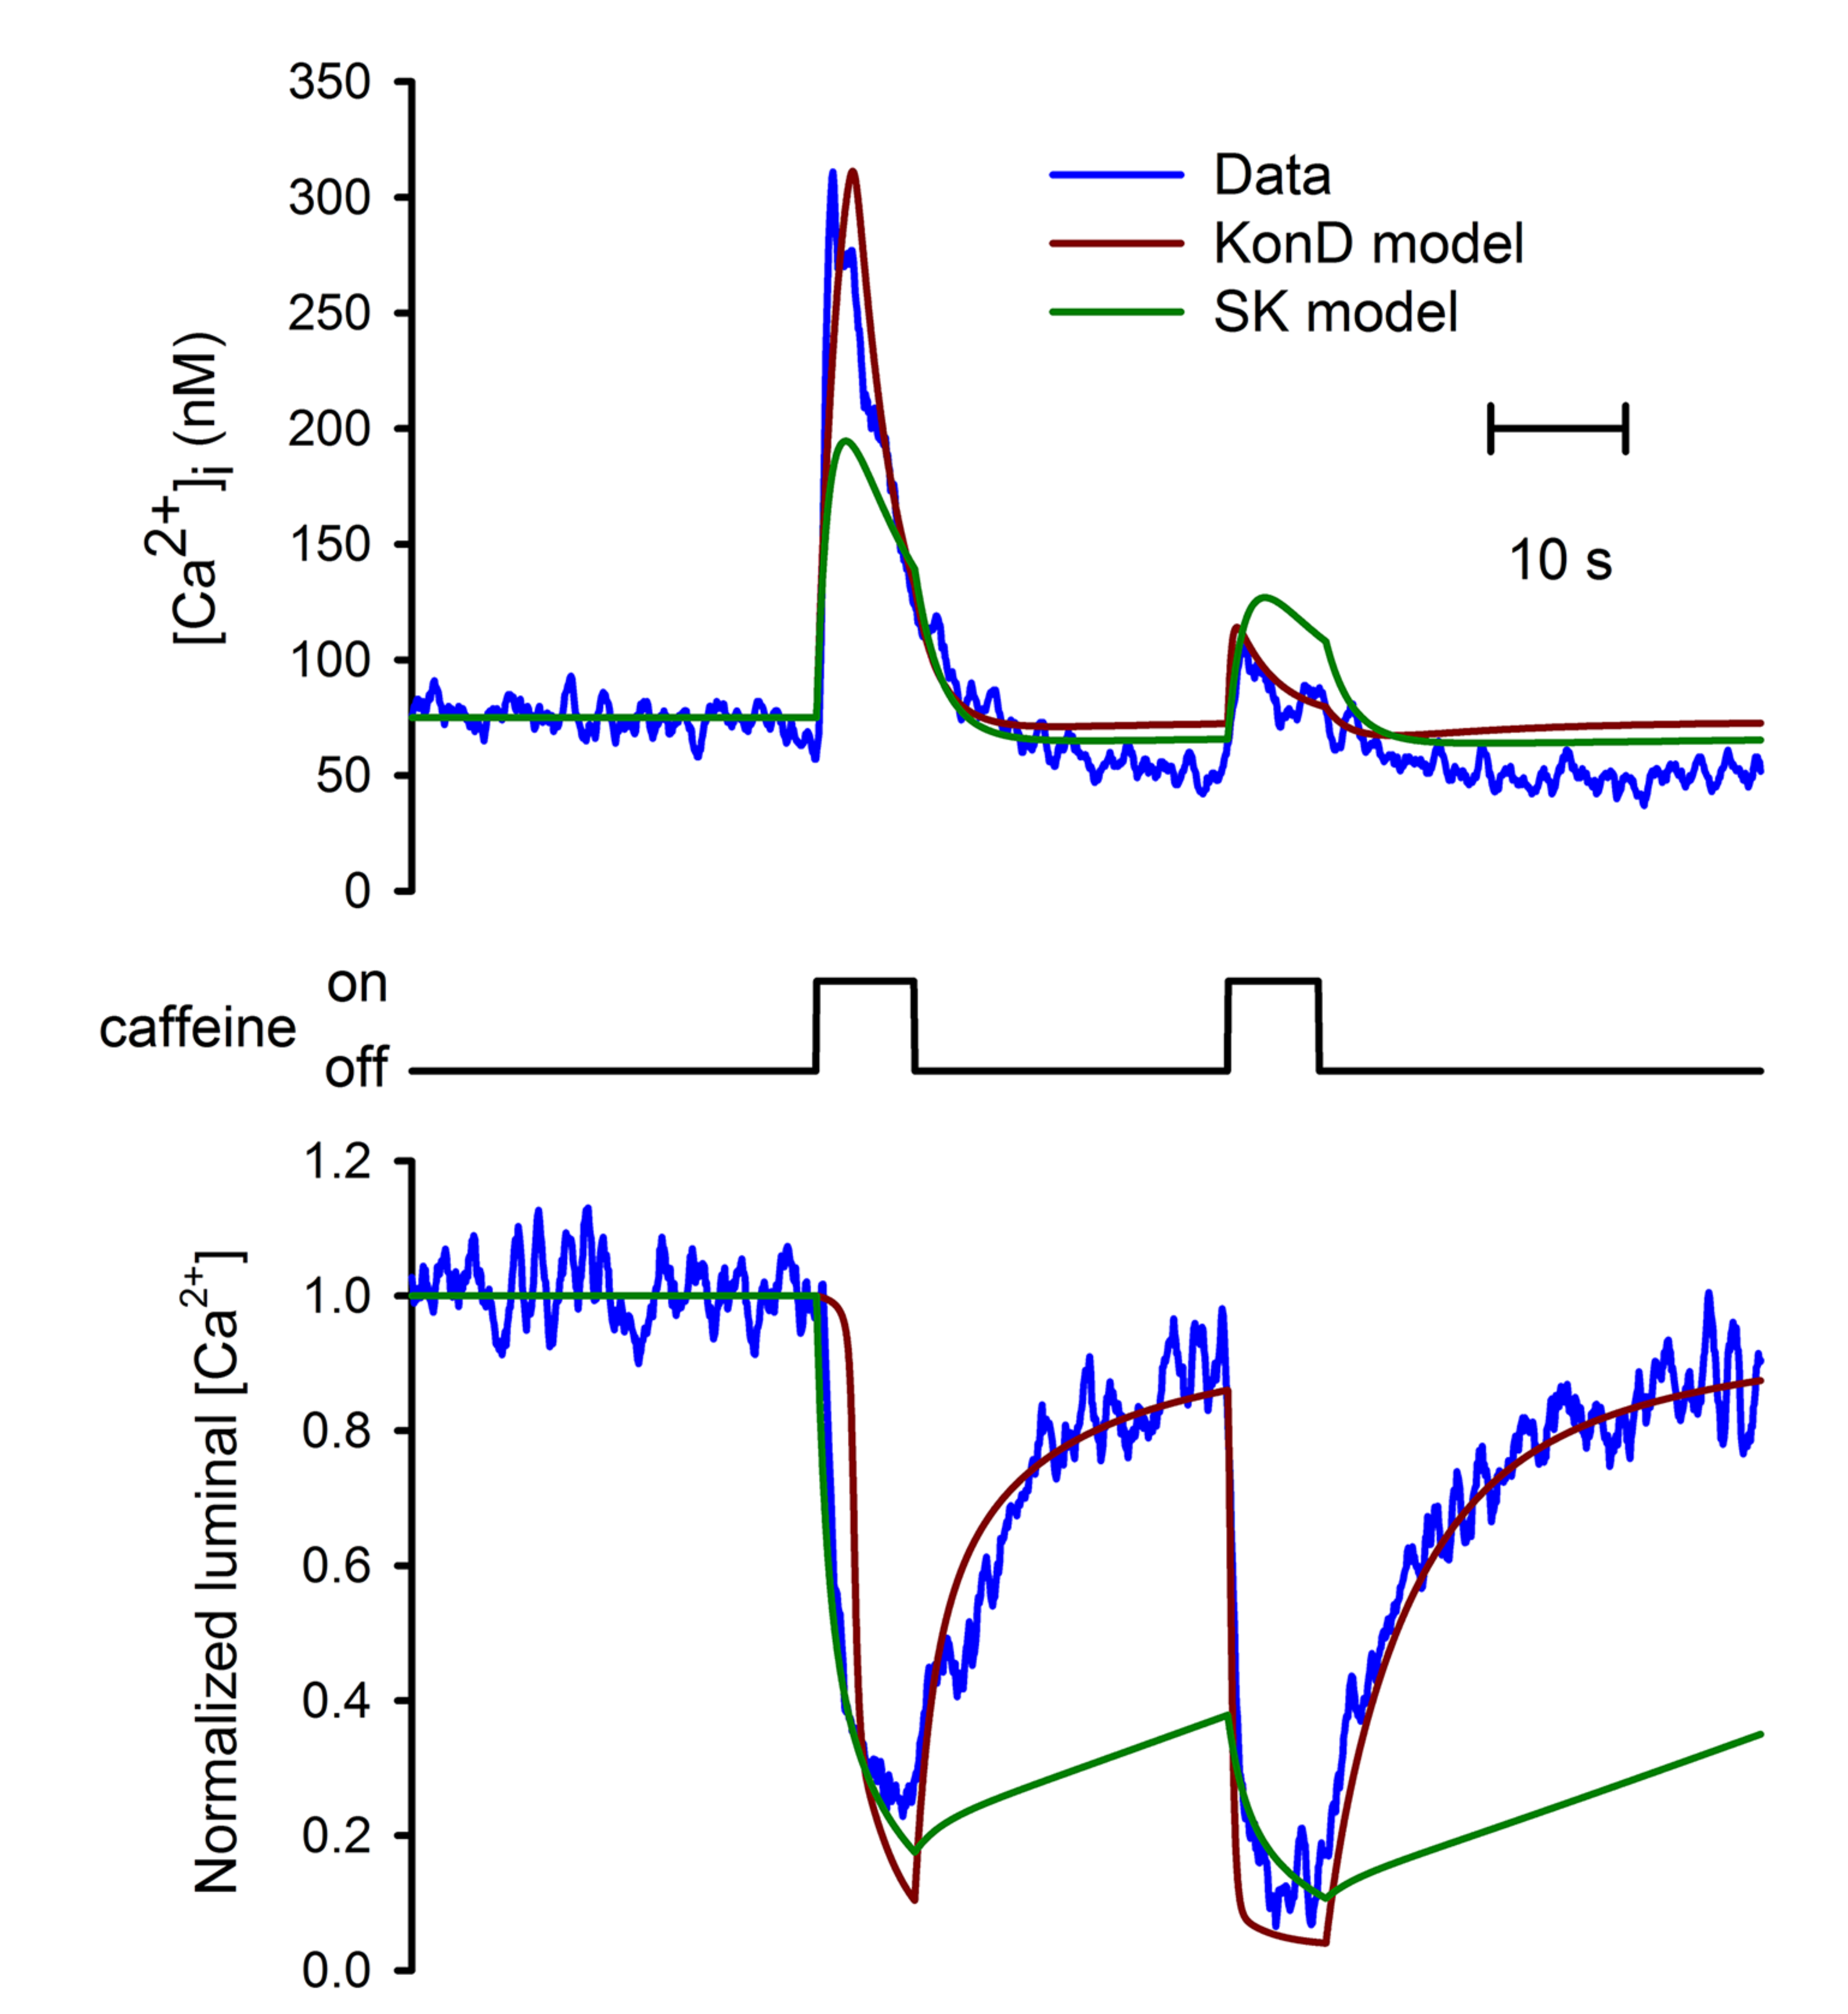
\includegraphics{FIGURA8}
	\caption{\textbf{Respuesta refractaria de los transitorios de calcio citoplásmico estimulados por cafeína.} Se muestran dos transitorios cada uno inducido por cafeína, los valores obtenidos experimentalmente, el ajuste bajo el modelo de SK y el ajuste con el modelo KonD. Imagen tomada de la referencia \cite{Perez-Rosas2015}.}
	\label{fig:FIGURA8}
\end{figure}

%------------------------------------------------

\section{Objetivos}

A pesar de que el modelo KonD parece ser una buena aproximación de la dinámica de calcio, en este trabajo se propone una alternativa a su hipótesis principal. Existe un número fijo de sitios de unión. Sin embargo, al polimerizarse la calsecuestrina, calcio adicional queda atrapado en los polímeros. De ahí que su capacidad amortiguadora aumente conforme aumentan la $\Cal$ y el grado de polimerización. Para el desarrollo de este trabajo nos propusimos los siguientes objetivos.

\subsection{Objetivo General}

Analizar la dinámica de la respuesta de calcio liberado por los RyRs en células de músculo liso.

\subsection{Objetivos Particulares}

\begin{itemize}
	\item Estudiar la dinámica de la polimerización de la calsecuestrina dependiente de calcio. \\
	
	\item Desarrollar un modelo matemático que relacione los cambios en la $\Cai$ y la $\Cal$ teniendo en cuenta la función de las proteínas amortiguadoras (calsecuestrina) dentro del retículo sarcoplásmico. \\
	
	\item Estudiar de manera analítica la estabilidad del modelo. \\
	
	\item Validar el modelo matemático con base en resultados experimentales.
\end{itemize}

%------------------------------------------------
\section{Metodología}

\subsection*{Lista de Variables y Parámetros}

\begin{itemize}
	\item $[Ca^{2+}]_{Ti}$ Concentración total de calcio intracelular ($nM$).
	\item $[Ca^{2+}]_{TSR}$ Concentración total de calcio luminal ($mM$).
	\item $\Cai$ Concentración de calcio intracelular libre ($nM$).
	\item $\Cal$ Concentración de calcio luminal libre ($\mu M$).
	\item $[\overline{Ca^{2+}}]_i$ Concentración basal de calcio intracelular ($nM$).
	\item $[\overline{Ca^{2+}}]_SR$ Concentración basal de calcio luminal ($\mu M$).
	\item $[Caff]$ Concentración de cafeína ($mM$).
	\item $\gamma$ Cociente entre el volumen del retículo y el volumen del citoplasma.
	\item $n_v$ Dimensión fractal del retículo sarcoplásmico.
	\item $a$ Constante de reacción de orden uno ($s^{-1}$).
	\item $b$ Constante proporcional al flujo máximo a través de un RyR ($s^{-1}$).
	\item $c$ Flujo máximo de calcio a través de las bombas SERCA ($nMs^{-1}$).
	
	
\end{itemize}

\subsection{Descripción del Modelo Matemático}

El modelo descrito a continuación es basado en el modelo desarrollado por Perez-Rosas \cite{Perez-Rosas2016}. Para desarrollar el modelo, consideraremos las células de músculo liso como dos compartimentos, el citoplasma y el retículo sarcoplásmico, y analizaremos el cambio de la concentración total de calcio en cada uno de ellos en función del tiempo como el flujo neto, \ie la diferencia entre el flujo de entrada y el flujo de salida, obteniendo lo siguiente

\begin{eqnarray}
\frac{d[Ca^{2+}]_{Ti}}{dt} & = & -J_{1}+J_{2}-J_{3}  \nonumber \\
\frac{d[Ca^{2+}]_{TSR}}{dt} & = & \frac{J_{3}-J_{2}}{\gamma}
\end{eqnarray}

$J_{1}$ representa el flujo producido por cualquier mecanismo de remoción en la membrana plasmática, \eg intercambiadores, bombas PMCA, y está dado por

\begin{equation}
J_{1}=a\left[[Ca^{2+}]_i - [\overline{Ca^{2+}}]_i\right]
\end{equation}

donde $a$ es la constante cinética de primer orden, $[Ca^{2+}]_i$ representa la concentración de calcio intracelular libre y $[\overline{Ca^{2+}}]_i$ es la concentración basal de calcio en citoplasma.

$J_{2}$ representa el flujo proveniente de los RyRs y está dado por

\begin{equation}
J_2=b\gamma^{n_v}P\left([Ca^{2+}]_i,[Caff]\right)\left[[Ca^{2+}]_{TSR}-[Ca^{2+}]_i\right]
\end{equation}

donde $b$ es un parámetro constante proporcional al flujo máximo a través de un RyR; $\gamma^{n_v}$ es la constante de proporcionalidad del número de RyR basada en la razón entre los volúmenes de la célula y del retículo, además el retículo parece ser una estructura fractal compleja y por lo tanto su superficie escala respecto al volumen de acuerdo con la ley de potencias $\gamma^{n_v}$ donde $n_v$ indica la dimensión fractal. Asumiendo que la densidad de RyR en la superficie del retículo es constante, el número de ellos será proporcional a $\gamma^{n_v}$; $P\left([Ca^{2+}]_i,[Caff]\right)$ es la probalidad de apertura de un RyR, que depende de la concentración de calcio en citoplasma y de la concentración de cafeína aplicada y está dada por

\begin{equation}
P\left([Ca^{2+}]_i, [Caff]\right)=\frac{[Ca^{2+}]_i\left(1 + k_f[Caff]\right)^{n_F}}{K^{n_F}_c + [Ca^{2+}]_i\left(1+k_f[Caff]\right)^{n_F}}
\end{equation}

aquí, $k_f = k_F/K_F$ donde $k_F$ representa la cooperatividad entre calcio y cafeína y $K_F$ es la constante de disociación del complejo RyR-Cafeína. $K_c$ es la constante de disociación del complejo RyR-calcio, $n_F$ es un coeficiente de Hill y la $\Cal$ está dada por la dinámica calcio-calsecuestrina. \\

$J_3$ representa el flujo a través de las bombas SERCA hacia el retículo sarcoplásmico y se encuentra dado por

\begin{equation}
J_3= c\frac{[Ca^{2+}]^{n_s}_i}{K^{n_s}_s+[Ca^{2+}]^{n_s}_i}
\end{equation}

donde $c$ representa el flujo máximo a través de las bombas SERCA, $K_s$ es la constante de saturación media y $n_s$ es un coeficiente de Hill.

\subsection{Estimación de los Parámetros}

Los parámetros serán tomados de la literatura. Aquellos que no se encuentren allí, serán estimados mediante simulaciones hechas en \textit{Python} ya sea por medio de barridos o de búsqueda heurística.

\subsection{Validación del Modelo Matemático}

El modelo se validará comparando los resultados obtenidos mediante simulación con los datos experimentales de \cite{Guerrero-Hernandez2010} y \cite{Perez-Rosas2015}.
%------------------------------------------------
\section{Avances}

Dimerización de calsecuestrina (trabajar en los tetrámeros).

%----------------------------------------------------------------------------------------

%	REFERENCE LIST
%----------------------------------------------------------------------------------------

\bibliographystyle{plain}
\bibliography{Calsequestrin-Calcium}

 


%----------------------------------------------------------------------------------------

\end{document}
